\documentclass[12pt]{article}

% ── Packages ──────────────────────────────────────────────────────────────────
\usepackage[margin=2.5cm]{geometry}
\usepackage{lmodern}
\usepackage[T1]{fontenc}
\usepackage[italian]{babel}
\usepackage{amsmath,amssymb}
\usepackage{booktabs}
\usepackage{graphicx}
\usepackage{hyperref}
\usepackage[round]{natbib}
\usepackage{float}
\usepackage{multirow}
\usepackage{caption}
\usepackage{subcaption}
\usepackage{xcolor}
\usepackage{enumitem}
\usepackage{microtype}
\usepackage{tikz}
\usetikzlibrary{arrows.meta, positioning, calc}

\hypersetup{
  colorlinks=true,
  linkcolor=blue!60!black,
  citecolor=blue!60!black,
  urlcolor=blue!60!black
}

% ── Custom commands ───────────────────────────────────────────────────────────
\newcommand{\arcsinh}{\operatorname{arcsinh}}

\title{Regimi quasi ortogonali in ISO New England:\\livello di prezzo e persistenza temporale come dimensioni indipendenti}

\author{
  Carlo Mari \and
  Cristiano Baldassari\textsuperscript{*} \\[0.5em]
  \textit{Universit\`a degli Studi della Tuscia} \\
  Viterbo, Italia \\[0.3em]
  \textsuperscript{*}Autore corrispondente: \texttt{cristiano.baldassari@unitus.it}
}

\date{Maggio 2026}

% ══════════════════════════════════════════════════════════════════════════════
\begin{document}
\maketitle

% ── Abstract ──────────────────────────────────────────────────────────────────
\begin{abstract}
I regimi del mercato elettrico vengono convenzionalmente descritti lungo una singola dimensione, il livello di prezzo.
Dimostriamo che questa visione trascura un intero asse della struttura di mercato.
Applicando una metodologia interamente non supervisionata e guidata dai dati, senza specificare a priori il numero di regimi né fornire etichette predefinite, a cinque anni di prezzi orari di ISO New England, scopriamo due assi quasi ortogonali di organizzazione dei regimi: è la struttura stessa dei dati a rivelare quanti regimi esistono e come si organizzano.
Un asse economico, derivato da statistiche descrittive specifiche del dominio, separa i regimi per livello di prezzo, dall'off-peak allo spike estremo invernale.
Un asse dinamico, derivato da una rete neurale pre-addestrata su centinaia di migliaia di serie temporali eterogenee e applicata senza alcun addestramento specifico sui dati elettrici, separa i regimi per persistenza temporale, dalla mean-reversion rapida agli stati in cui gli shock perdurano per giorni.
I due assi sono praticamente indipendenti: conoscere il regime di prezzo non fornisce quasi alcuna informazione sul regime dinamico, e viceversa.
All'interno dello stesso regime economico, la velocità di mean-reversion varia di un fattore~5 a seconda del regime dinamico, un'eterogeneità invisibile a qualsiasi modello che descriva il mercato con un'unica etichetta di stato.
La struttura bidimensionale consente di costruire un modello mean-reverting condizionato a entrambi gli assi, in cui ogni combinazione prezzo--persistenza riceve i propri parametri: il guadagno informativo rispetto al modello convenzionale a un solo asse è statisticamente schiacciante e apre la strada a strategie di copertura e previsione che distinguono non solo \emph{quanto} costa l'elettricità, ma anche \emph{quanto a lungo} lo shock persisterà.

\medskip
\noindent\textbf{Parole chiave:} mercati elettrici spot, rilevamento non supervisionato dei regimi, analisi topologica dei dati, foundation model per serie temporali, diffusion maps
\end{abstract}

\newpage

% ══════════════════════════════════════════════════════════════════════════════
\section{Introduzione}
\label{sec:introduction}

Il mercato elettrico è organizzato lungo due assi quasi ortogonali, non uno.
Oltre al livello di prezzo, l'unica dimensione catturata dai modelli convenzionali, esiste un asse di persistenza temporale che determina quanto a lungo uno shock si propaga nel sistema.
I due assi sono quasi ortogonali: conoscere il regime di prezzo non dice quasi nulla sulla velocità di mean-reversion, e viceversa.
Questo lavoro scopre questa struttura bidimensionale attraverso una pipeline non supervisionata e ne quantifica le conseguenze per la modellazione e la gestione del rischio.

% --- 1.1 Il contesto economico ---

L'elettricità non può essere immagazzinata a costi ragionevoli: l'offerta deve eguagliare la domanda in ogni istante, e il prezzo riflette il costo dell'ultimo generatore necessario per mantenere il sistema in equilibrio.
I generatori vengono ordinati per costo di produzione in una graduatoria nota come merit order: quando la domanda è bassa i generatori economici sono sufficienti e i prezzi sono bassi, quando la domanda sale o l'offerta diminuisce il sistema ricorre a unità progressivamente più costose e il prezzo sale di conseguenza \citep{weron2014}.
Negli Stati Uniti, i mercati elettrici all'ingrosso sono gestiti da Independent System Operators (ISO) che compensano domanda e offerta attraverso aste centralizzate producendo un Locational Marginal Price (LMP) per ogni nodo della rete.
Questo lavoro si concentra su ISO New England (ISONE), ma la metodologia è applicabile a qualsiasi mercato nodale che produca LMP orari.

La serie LMP presenta proprietà statistiche che la distinguono dalla maggior parte degli asset finanziari: code pesanti, mean-reversion a scale temporali multiple, tre cicli stagionali sovrapposti (giornaliero, settimanale, annuale) e valori occasionalmente negativi \citep{ziel2018, weron2006}.
Identificare il regime di mercato prevalente ha conseguenze pratiche dirette per la copertura del rischio \citep{coulon2014}, la pianificazione della capacità e la previsione dei prezzi \citep{janczura2013, nowotarski2018}.

% --- 1.2 Approcci esistenti e loro limiti ---

Il rilevamento non supervisionato dei regimi nei mercati elettrici resta una sfida aperta \citep{weron2014}.
La letteratura ha affrontato il problema con tre famiglie principali di modelli.
Gli Hidden Markov Models (HMM) \citep{mount2006, hamilton1989} e i Gaussian Mixture Models (GMM) \citep{kanamura2009} richiedono di specificare il numero di stati \emph{a priori} e assumono distribuzioni parametriche che mal si adattano alle code pesanti dei prezzi elettrici \citep{bierbrauer2007}.
I modelli mean-reverting a salti \citep{lucia2002, cartea2005} catturano la tendenza dei prezzi a tornare verso un livello di equilibrio, ma vincolano la velocità di mean-reversion a essere omogenea o al più modulata dal regime di prezzo.
Lavori più recenti hanno esplorato K-means e clustering spettrale \citep{rintamaki2017}, ma dipendono ancora da un $K$ pre-specificato.

Questi approcci condividono un limite profondo: ciascuna famiglia cattura implicitamente una dimensione diversa del mercato (HMM e GMM separano i \emph{livelli di prezzo}, i modelli mean-reverting descrivono la \emph{dinamica temporale}), ma nessuno si chiede se queste dimensioni siano governate dallo stesso processo latente o da processi indipendenti.
La letteratura ha documentato che entrambe presentano struttura propria: il volatility clustering \citep{cont2001} è presente nei prezzi elettrici, gli spike si aggregano in cluster persistenti \citep{christensen2009}, e la velocità con cui il mercato assorbe uno shock varia nel tempo e tra condizioni operative diverse \citep{karakatsani2008, knittel2005}.
Eppure, un'unica etichetta di stato continua a collassare livello e dinamica in una sola variabile.

Un mercato a \$100/MWh che tornerà a \$50 entro poche ore pone un rischio diverso da un mercato a \$100/MWh che resterà elevato per due settimane, eppure un'unica etichetta ``spike'' confonde i due casi \citep{huisman2003}.
La letteratura ha accumulato evidenza che sia la volatilità sia la persistenza presentano una struttura propria, ma non ha mai verificato se questa struttura sia indipendente dal livello di prezzo.
Questo lavoro colma questo gap.

% --- 1.3 Nuovi strumenti ---

Due sviluppi recenti creano l'opportunità di testare questa ipotesi.
Primo, i foundation model per serie temporali \citep{yeh2023}: reti neurali di grandi dimensioni addestrate su centinaia di migliaia di serie temporali eterogenee (meteorologia, finanza, sanità, ingegneria), riutilizzabili su qualsiasi nuova serie senza addestramento aggiuntivo.
La diversità di pattern osservati durante il pre-addestramento (trend, stagionalità, persistenza, cambi di regime) viene condensata nei parametri della rete, creando un patrimonio di conoscenze trasferibile a qualsiasi dominio \citep{tsfm_survey2025}.
Non è necessario decidere cosa cercare: è il modello a trovare ciò che i dati contengono.
Tra i foundation model disponibili, adottiamo MOMENT \citep{moment2024} perché soddisfa tre requisiti: è progettato per serie temporali (non adattato da modelli linguistici), fornisce una modalità nativa di embedding per l'apprendimento delle rappresentazioni (non solo per la previsione), ed è interamente open source.
MOMENT è particolarmente adatto perché, tra i foundation model disponibili al momento dello studio (Chronos, TimesFM, Moirai), è l'unico a soddisfare contemporaneamente tutti e tre i requisiti.
Secondo, l'analisi topologica dei dati \citep{carlsson2009, edelsbrunner2010} offre metodi di clustering che determinano il numero di regimi direttamente dalla geometria dei dati, senza specificare $K$ in anticipo.
Ad oggi, i foundation model sono stati applicati ai mercati elettrici solo per la previsione dei prezzi \citep{tsfm_epf_benchmark2025, pricefm2025} e il rilevamento di anomalie \citep{tsfm_anomaly_energy2024}; l'approccio qui proposto, utilizzare le loro rappresentazioni come input per un clustering non supervisionato, non ha precedenti nella letteratura sui mercati energetici.

% --- 1.4 Strategia e contributo ---

La strategia consiste nel costruire due rappresentazioni degli stessi dati di prezzo, una basata su statistiche specifiche del dominio e una su un foundation model, e nel clusterizzare ciascuna indipendentemente con lo stesso algoritmo non parametrico.
Le due rappresentazioni derivano dalla stessa serie di residui attraverso una trasformazione deterministica e invertibile: se il mercato fosse organizzato lungo una sola dimensione, entrambe le viste la catturerebbero e le partizioni risulterebbero concordi.

Il contributo è triplice.
Primo, scopriamo un asse della struttura di mercato, la persistenza temporale, che è statisticamente indipendente dal livello di prezzo.
Secondo, il numero di regimi non è specificato a priori ma emerge dalla struttura dei dati attraverso una pipeline non supervisionata (Figura~\ref{fig:pipeline}).
Terzo, l'asse dinamico è scoperto da MOMENT applicato senza alcun addestramento sui dati elettrici: il modello riceve esclusivamente i residui destagionalizzati $r_t$, senza accesso al livello di prezzo, e qualsiasi struttura catturi proviene dalla dinamica temporale della serie.

La pipeline (Figura~\ref{fig:pipeline}) preprocessa la serie oraria dei prezzi~(a), costruisce le due rappresentazioni~(b,c), riduce ciascuna a poche coordinate tramite Diffusion Maps~(d), identifica i modi di densità con ToMATo~(e), determina la variabile di merge tramite una diagnostica di separazione~(f), e consolida i modi tramite Tukey HSD~(g).

% ── Diagramma della pipeline ─────────────────────────────────────────────────
\begin{figure}[H]
\centering
\resizebox{0.65\textwidth}{!}{%
\begin{tikzpicture}[
  font=\small,
  >=Latex,
  node distance=0.75cm,
  box/.style={
    draw=black!60, thick, rounded corners=3pt,
    minimum width=4.5cm, minimum height=0.85cm,
    align=center, font=\small
  },
  arr/.style={->, thick, black!60}
]

% Nodes
\node[box, fill=gray!10] (lmp) {\textbf{LMP orario}};

\node[box, fill=green!8, below=of lmp] (pre) {\textbf{Preprocessing}};

% Fork — wider spread
\node[box, fill=yellow!12, below left=1.2cm and 1.8cm of pre] (fe) {\textbf{Feature Engineering}};
\node[box, fill=blue!10, below right=1.2cm and 1.8cm of pre] (mom) {\textbf{Encoder MOMENT}};

\coordinate[below=0.6cm of pre] (fork);

\node[box, fill=purple!8, below=3.0cm of pre] (dm) {\textbf{Diffusion Maps}};

\node[box, fill=green!10, below=of dm] (tomato) {\textbf{Clustering ToMATo}};

\node[box, fill=cyan!8, below=of tomato, text width=5cm] (cross) {\textbf{Diagnostica di separazione}};

\node[box, fill=orange!10, below=of cross] (tukey) {\textbf{Merge Tukey HSD}};

\node[box, fill=gray!6, below=of tukey] (regimes) {\textbf{Regimi finali}};

\node[box, fill=yellow!10, draw=red!50, dashed, thick, below=of regimes]
  (axes) {\textcolor{red!65!black}{\textbf{Due assi quasi ortogonali}}};

% Arrows — main flow
\draw[arr] (lmp) -- (pre);

% Fork: pre → horizontal bar → down to FE and MOM
\draw[thick, black!60] (pre.south) -- (fork);
\coordinate (fork_l) at (fe.north |- fork);
\coordinate (fork_r) at (mom.north |- fork);
\draw[thick, black!60] (fork_l) -- (fork_r);
\draw[arr] (fork_l) -- (fe.north);
\draw[arr] (fork_r) -- (mom.north);

% Merge: FE and MOM → down → horizontal bar → down to DM
\coordinate (merge_l) at ([yshift=-0.5cm]fe.south);
\coordinate (merge_r) at ([yshift=-0.5cm]mom.south);
\draw[thick, black!60] (fe.south) -- (merge_l);
\draw[thick, black!60] (mom.south) -- (merge_r);
\draw[thick, black!60] (merge_l) -- (merge_r);
\coordinate (merge_mid) at ($(merge_l)!0.5!(merge_r)$);
\draw[arr] (merge_mid) -- (dm.north);

\draw[arr] (dm) -- (tomato);
\draw[arr] (tomato) -- (cross);
\draw[arr] (cross) -- (tukey);
\draw[arr] (tukey) -- (regimes);
\draw[arr, dashed, red!50!black] (regimes) -- (axes);

% Alphabetic labels on the left
\node[font=\scriptsize\bfseries, gray, left=0.4cm] at (pre.west) {(a)};
\node[font=\scriptsize\bfseries, gray, left=0.4cm] at (fe.west) {(b)};
\node[font=\scriptsize\bfseries, gray, right=0.4cm] at (mom.east) {(c)};
\node[font=\scriptsize\bfseries, gray, left=0.4cm] at (dm.west) {(d)};
\node[font=\scriptsize\bfseries, gray, left=0.4cm] at (tomato.west) {(e)};
\node[font=\scriptsize\bfseries, gray, left=0.4cm] at (cross.west) {(f)};
\node[font=\scriptsize\bfseries, gray, left=0.4cm] at (tukey.west) {(g)};

\end{tikzpicture}%
}
\caption{Pipeline non parametrica per il rilevamento dei regimi. Per chiarezza il diagramma mostra un singolo ramo; i passi (d)--(g) vengono applicati indipendentemente a ciascuna rappresentazione, producendo due partizioni distinte.}
\label{fig:pipeline}
\end{figure}

Il codice completo della pipeline e gli script di elaborazione dati sono pubblicamente disponibili all'indirizzo \url{https://github.com/cbaldassari/two-axes}.

Il resto del lavoro è organizzato come segue.
La Sezione~\ref{sec:data} descrive i dati e il preprocessing.
La Sezione~\ref{sec:pipeline} presenta le due rappresentazioni e il clustering non parametrico.
La Sezione~\ref{sec:results} dimostra che i due assi sono indipendenti e quantifica le conseguenze economiche della struttura bidimensionale.
La Sezione~\ref{sec:discussion} discute le implicazioni operative e le limitazioni.
La Sezione~\ref{sec:conclusion} conclude.

\section{Dati}
\label{sec:data}

% ── 2.1 Dati e preprocessing ──────────────────────────────────────────────────
\subsection{Dati e preprocessing}
\label{sec:preprocessing}

Gli LMP orari day-ahead per il Massachusetts Hub di ISO New England vengono scaricati dalla U.S.\ Energy Information Administration (EIA).\footnote{EIA Open Data API v2: \url{https://api.eia.gov/v2/electricity/rto/wholesale-data}. Parametri di query: \texttt{respondent=ISNE}, \texttt{type=D} (day-ahead). È necessaria una chiave API gratuita, ottenibile su \url{https://www.eia.gov/opendata/register.php}.}
Il Locational Marginal Price (LMP) è il prezzo all'ingrosso dell'elettricità in un nodo specifico della rete di trasmissione, determinato ogni ora attraverso un'asta competitiva in cui i generatori presentano offerte di vendita e l'operatore di sistema compensa il mercato.
Il Massachusetts Hub è un nodo di prezzo di riferimento ampiamente utilizzato come benchmark per la regione del New England.

Il campione contiene 43\,814 osservazioni orarie che coprono il periodo da gennaio 2021 a dicembre 2025 (Tabella~\ref{tab:lmp_stats}).
Questa finestra quinquennale cattura diversi episodi di mercato distinti: la ripresa della domanda post-COVID (2021), lo spike del prezzo del gas naturale causato dal conflitto Russia--Ucraina (2022), la successiva normalizzazione (2023--2024), e diversi eventi estremi di freddo invernale che hanno innescato spike di prezzo superiori a \$400/MWh.

\begin{table}[H]
\centering
\caption{Statistiche descrittive dell'LMP del Massachusetts Hub ISONE (\$/MWh), 2021--2025.}
\label{tab:lmp_stats}
\small
\begin{tabular}{lrlr}
\toprule
\multicolumn{2}{c}{\textit{Campione}} & \multicolumn{2}{c}{\textit{Distribuzione}} \\
\cmidrule(lr){1-2} \cmidrule(lr){3-4}
Osservazioni    & 43\,814     & Media        & 55,51  \\
Valori mancanti & 0           & Mediana      & 41,05  \\
Periodo         & 2021--2025  & Dev.\ std    & 42,37  \\
Frequenza       & oraria      & Asimmetria   & 2,34   \\
                &             & Curtosi      & 9,94   \\
\cmidrule(lr){1-2} \cmidrule(lr){3-4}
\multicolumn{2}{c}{\textit{Range e percentili}} & \multicolumn{2}{c}{\textit{Valori estremi}} \\
\cmidrule(lr){1-2} \cmidrule(lr){3-4}
Minimo          & 9,15        & Oss.\ $> 400$ & 4     \\
$Q_5$           & 20,22       & Oss.\ $< 10$  & 4     \\
$Q_{25}$        & 28,82       & Oss.\ $< 0$   & 0     \\
$Q_{75}$        & 64,96       & Oss.\ $= 0$   & 0     \\
$Q_{95}$        & 151,90      &               &       \\
Massimo         & 474,90      &               &       \\
\bottomrule
\end{tabular}
\par\smallskip
\footnotesize\textit{Nota:} Tutti i valori in \$/MWh tranne dove indicato. Curtosi di Pearson (gaussiana~$= 3$).
\end{table}

I prezzi dell'elettricità coprono un ampio intervallo: nel nostro campione vanno da un minimo di \$9/MWh a un massimo di quasi \$475/MWh, con una forte asimmetria positiva (mediana \$41 contro media \$56) e code pesanti (curtosi 9,94, oltre tre volte il valore gaussiano).
In generale, i prezzi LMP possono assumere valori negativi durante periodi di eccesso di generazione rinnovabile, sebbene nel nostro campione non si osservino episodi di prezzo negativo.
Per stabilizzare la varianza preservando al contempo l'intero supporto della distribuzione, applichiamo la trasformazione arco-seno iperbolico,
\begin{equation}
y_t = \arcsinh(p_t) = \ln\!\left(p_t + \sqrt{p_t^2 + 1}\right),
\label{eq:arcsinh}
\end{equation}
che è definita su tutto $\mathbb{R}$, non richiede parametri di regolazione, e ha un utile comportamento duale: per $|p|$ grandi agisce come $\log(2|p|)$, comprimendo gli spike estremi; vicino allo zero è approssimativamente lineare, preservando la struttura fine dei movimenti di prezzo nel regime normale.
Questa trasformazione stabilizza la varianza ma non rende la serie stazionaria: trend e stagionalità sono ancora presenti e devono essere rimossi nel passo successivo.

La serie trasformata $y_t$ presenta una forte stagionalità a tre scale: 24\,h (ciclo domanda giorno/notte), 168\,h (schema giorno feriale/fine settimana), e 8\,760\,h (ciclo annuale estate/inverno).
Se non rimossa, queste componenti stagionali dominano il clustering, che finirebbe per riscoprire semplicemente ``estate contro inverno'' piuttosto che regimi strutturali di mercato.
Applichiamo MSTL (Multi-Seasonal-Trend decomposition using Loess) \citep{bandara2021}, una generalizzazione di STL \citep{cleveland1990} che gestisce simultaneamente più periodi stagionali.
STL decompone una serie temporale in trend, una componente stagionale e residuo usando regressione ponderata localmente (Loess); MSTL estende questo a un numero arbitrario di periodi stagionali estraendo iterativamente ciascun ciclo:
\begin{equation}
y_t = \tau_t + s_t^{(24)} + s_t^{(168)} + s_t^{(8760)} + r_t,
\label{eq:mstl}
\end{equation}
dove $\tau_t$ è il trend, $s_t^{(P)}$ è la componente stagionale al periodo $P$, e $r_t$ è il residuo --- il segnale destagionalizzato che serve come input per il rilevamento dei regimi.
I tre periodi stagionali sono:

\begin{table}[H]
\centering
\small
\begin{tabular}{clc}
\toprule
$P$ (ore) & Ciclo & Causa \\
\midrule
24    & Giornaliero & Domanda giorno/notte \\
168   & Settimanale  & Domanda feriale/festivo \\
8\,760 & Annuale  & Raffrescamento estivo / riscaldamento invernale \\
\bottomrule
\end{tabular}
\end{table}
La Figura~\ref{fig:mstl} mostra tutte e cinque le componenti.

\begin{table}[H]
\centering
\caption{Statistiche descrittive del residuo MSTL $r_t$.}
\label{tab:residual_stats}
\begin{tabular}{lcccc}
\toprule
& Media & Dev.\ std & Asimmetria & Curtosi \\
\midrule
Residuo MSTL $r_t$ & 0,005 & 0,286 & 0,21 & 4,50 \\
\bottomrule
\end{tabular}
\par\smallskip
\footnotesize\textit{Nota:} Curtosi di Pearson; una distribuzione gaussiana ha curtosi~3.
\end{table}

\noindent Il residuo presenta code sostanzialmente più leggere rispetto all'LMP grezzo (curtosi 4,50 vs.\ 9,94), confermando che la trasformazione arcsinh e la rimozione stagionale hanno assorbito la maggior parte della variazione estrema.

\begin{figure}[H]
\centering
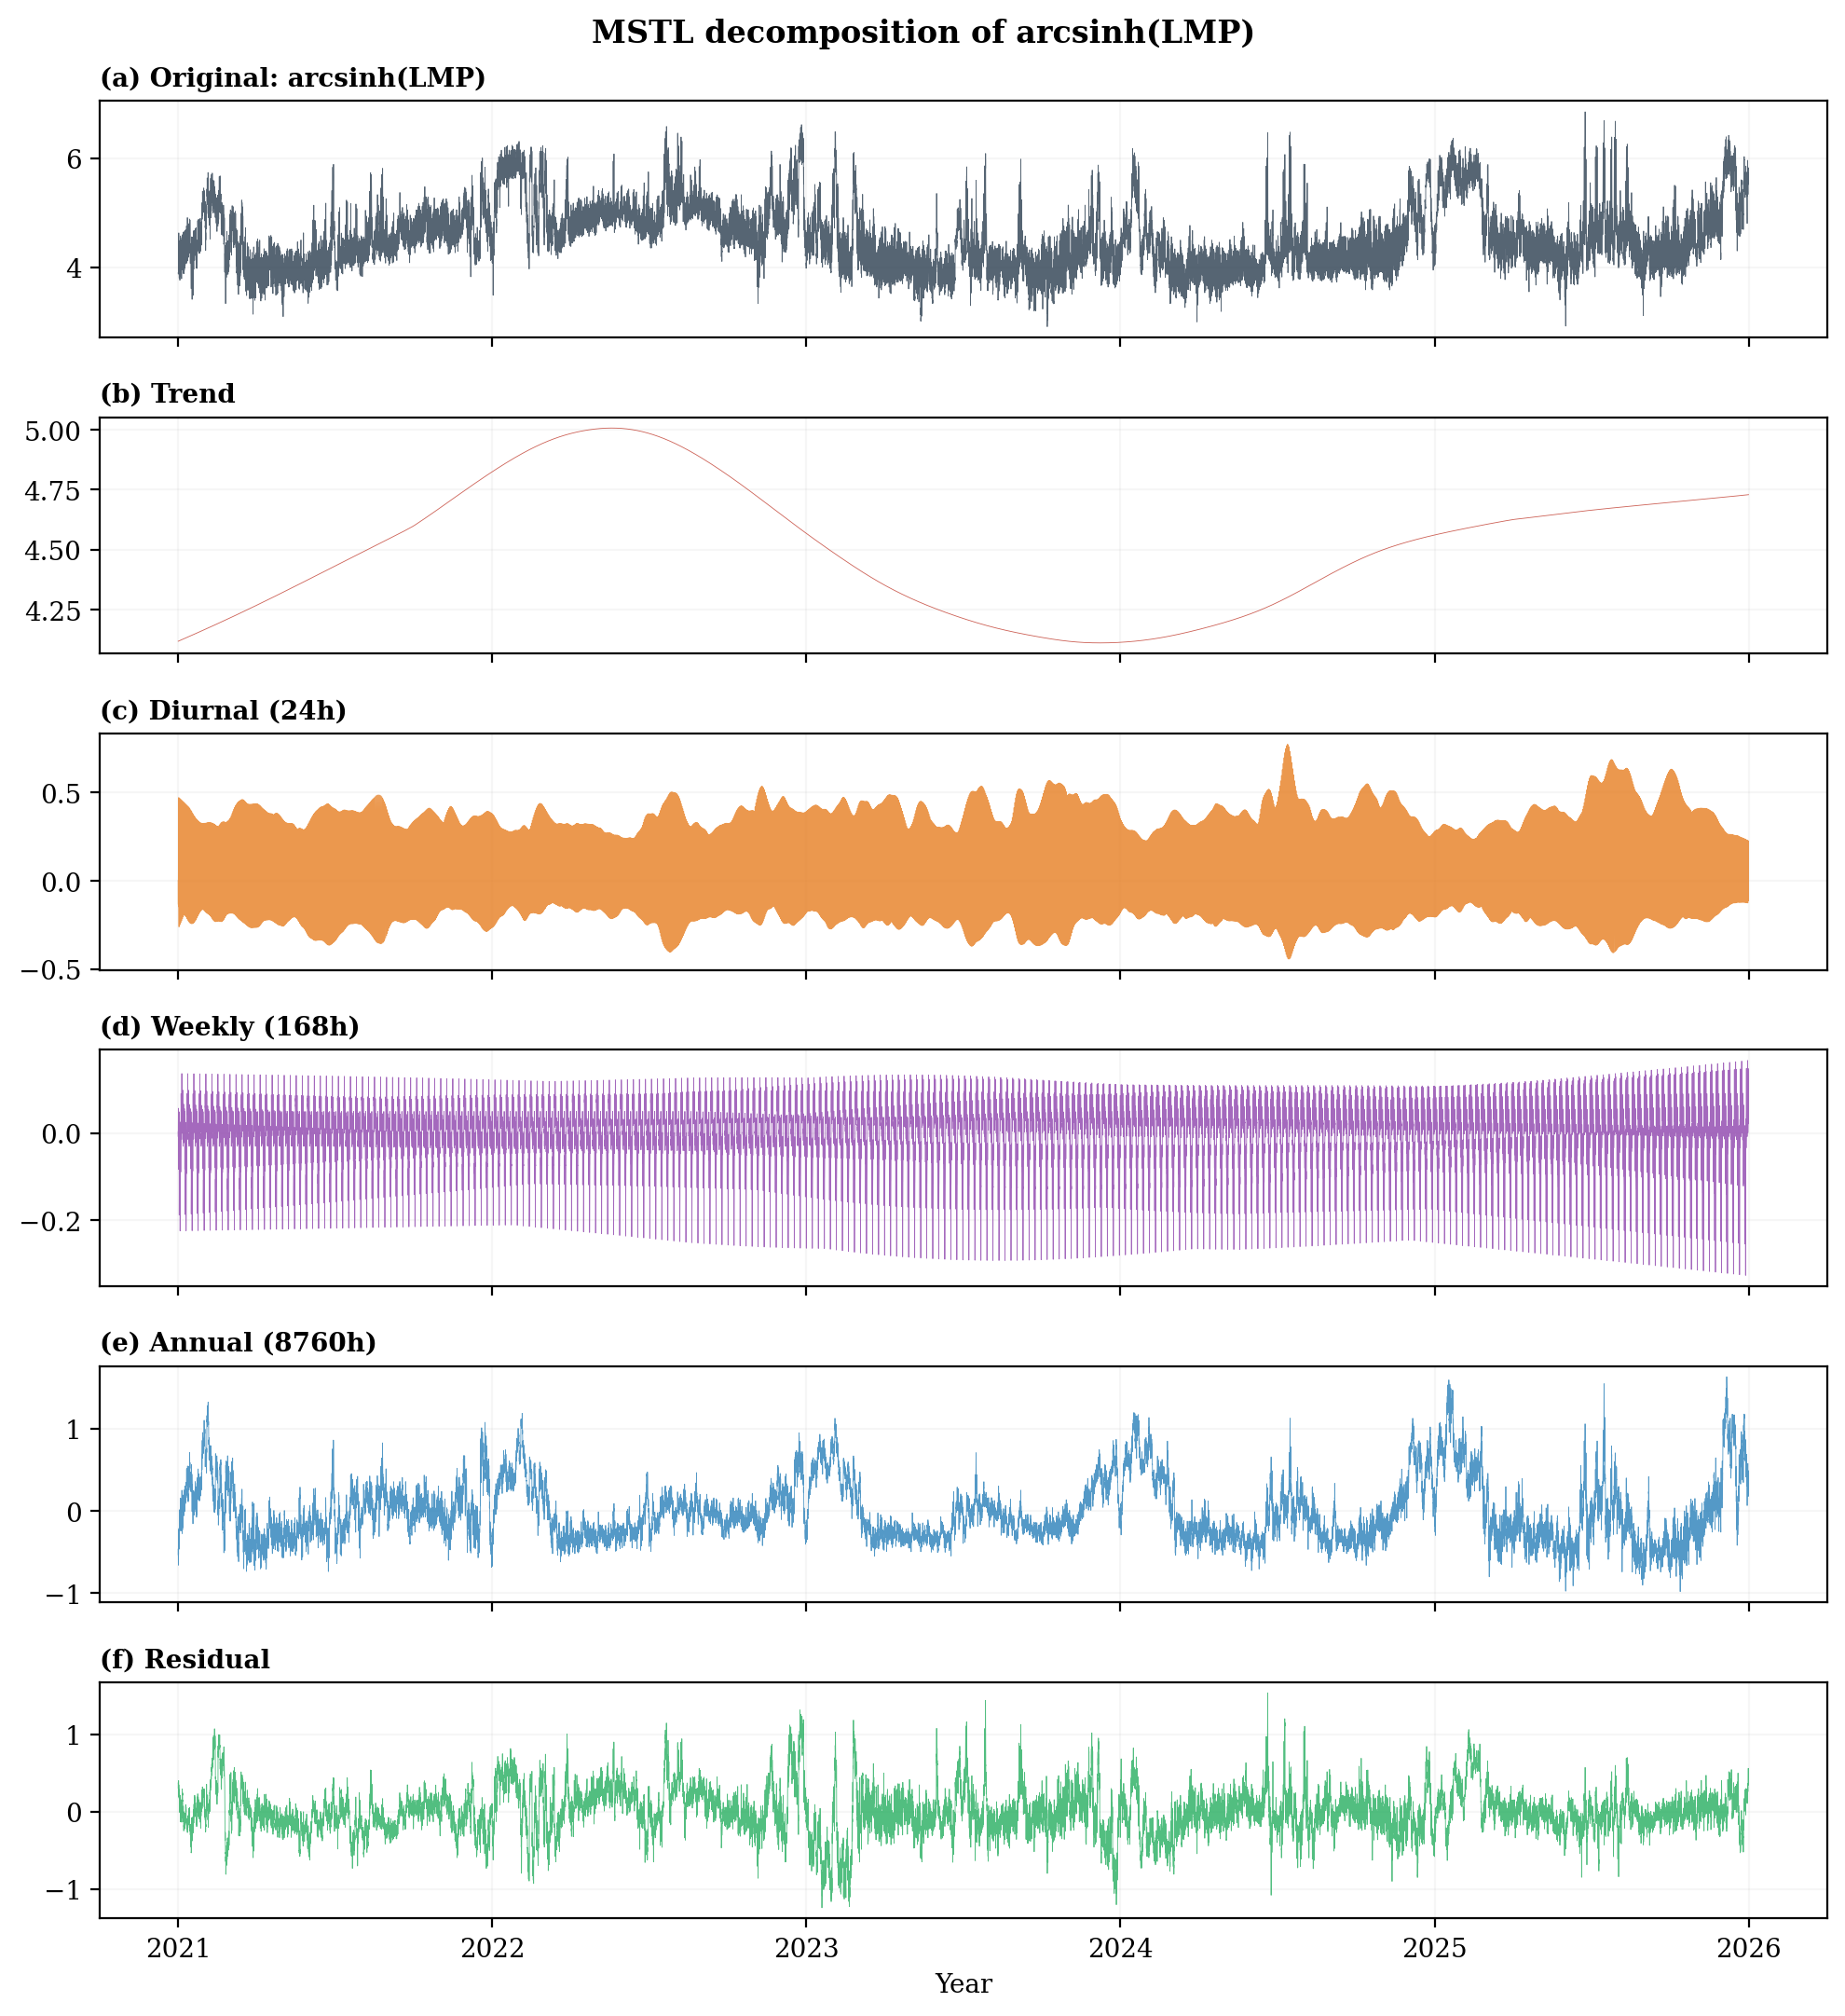
\includegraphics[width=0.68\textwidth]{mstl_decomposition.png}
\caption{Decomposizione MSTL di arcsinh(LMP). (a) serie originale; (b) trend; (c) stagionalità giornaliera; (d) stagionalità settimanale; (e) stagionalità annuale; (f) residuo.}
\label{fig:mstl}
\end{figure}

Per verificare l'efficacia della destagionalizzazione esaminiamo la funzione di autocorrelazione (ACF).
La Tabella~\ref{tab:acf} mostra che l'ACF al lag 24 scende da 0,890 a 0,770 e quella al lag 168 da 0,678 a 0,238: la decomposizione MSTL attenua le componenti stagionali ma il residuo conserva una fortissima persistenza oraria ($\text{ACF lag~1} = 0{,}977$).
Questa persistenza residua non è un'imperfezione del filtraggio: è la \emph{materia prima stocastica} del mercato.
Una volta rimosse le componenti cicliche deterministiche, ciò che resta è la memoria del processo --- quanto velocemente il mercato assorbe uno shock --- e la sua intensità varia nel tempo.
Come vedremo nella Sezione~\ref{sec:model_insufficiency}, è proprio la variabilità di questa persistenza a costituire l'informazione che i modelli che descrivono il mercato con un'unica etichetta di regime faticano ad allocare.

\begin{table}[H]
\centering
\caption{Autocorrelazione prima e dopo la decomposizione MSTL.}
\label{tab:acf}
\begin{tabular}{lcccc}
\toprule
& Lag 1 & Lag 24 & Lag 168 & Lag 8760 \\
\midrule
arcsinh(LMP)     & 0,974 & 0,890 & 0,678 & 0,108 \\
Residuo MSTL     & 0,977 & 0,770 & 0,238 & $-$0,403 \\
\bottomrule
\end{tabular}
\end{table}

MSTL viene applicato globalmente all'intera serie di 43\,814 ore prima di qualsiasi finestratura, producendo un'unica sequenza di residui orari $r_1, r_2, \ldots, r_{43814}$.

\subsection{Due viste dello stesso residuo}
\label{sec:two_views}

Il residuo $r_t$ è un processo stocastico con forte persistenza (ACF lag~1 $= 0{,}977$).
Nella teoria dei processi stocastici, un processo può essere descritto attraverso due rappresentazioni complementari:
\begin{itemize}[nosep]
\item I suoi \textbf{livelli} $r_t$: descrivono la struttura di dipendenza temporale --- come gli shock si propagano, quanto il processo è persistente, se e quanto velocemente avviene la mean-reversion.
\item I suoi \textbf{incrementi} $\Delta r_t = r_t - r_{t-1}$: descrivono la distribuzione delle innovazioni --- quanto sono ampi gli shock, se sono simmetrici, se hanno code pesanti. La serie $\Delta r_t$ è stazionaria.
\end{itemize}

Le due rappresentazioni sono deterministicamente derivate dalla stessa serie e coprono le stesse finestre temporali.
Non sono ``dati diversi'' --- sono due viste dello stesso fenomeno, come descrivere il moto di un corpo tramite la posizione (dove si trova nel tempo) o la velocità (quanto cambia posizione ad ogni istante).

Questa distinzione è importante perché i due strumenti di rappresentazione che utilizziamo (Sezione~\ref{sec:pipeline}) hanno requisiti computazionali diversi.
Le \textbf{statistiche distribuzionali} (media, varianza, curtosi, percentili) sono invarianti all'ordine temporale --- rimescolando i valori nella finestra, si ottengono gli stessi numeri.
Per essere stimatori consistenti della distribuzione marginale delle innovazioni, richiedono un input stazionario: ricevono $\Delta r_t$.
L'\textbf{encoder temporale} (MOMENT) è un modello di sequenza che processa i valori nel loro ordine: la persistenza del processo è il segnale che deve codificare, non un disturbo da eliminare.
Se l'input fosse rumore bianco ($\Delta r_t$), tutte le finestre produrrebbero embedding indistinguibili: MOMENT riceve $r_t$.

Un regime di mercato non è un evento istantaneo: è uno stato sostenuto che persiste per giorni o settimane.
Un singolo residuo orario $r_t$ ci dice la deviazione di prezzo in un istante, ma non può dirci se il mercato è volatile o calmo, se gli shock persistono o rientrano rapidamente.
Queste proprietà possono essere osservate solo su un blocco esteso di ore consecutive.
La sequenza dei residui viene quindi suddivisa in finestre scorrevoli sovrapposte, ciascuna composta da $W$ residui orari consecutivi.

La lunghezza della finestra è $W = 512$ ore ($\approx$ 21 giorni), determinata dal vincolo architetturale di MOMENT il cui contesto massimo è 512 token (Sezione~\ref{sec:repr_moment}); questa lunghezza copre almeno tre cicli settimanali completi.
Il passo $S = 6$ ore bilancia due esigenze contrapposte: da un lato, un passo piccolo garantisce una risoluzione temporale fine, permettendo di osservare quando il mercato transita da un regime all'altro senza perdere transizioni rapide; dall'altro, un passo troppo piccolo produrrebbe finestre quasi identiche tra loro (con 512 ore in comune su 512), inflazionando la dimensione campionaria senza aggiungere informazione reale.
Con $S = 6$, ogni nuova finestra differisce dalla precedente per sole 6 ore su 512, ma quattro finestre al giorno sono sufficienti per risolvere le dinamiche di regime alla scala sub-giornaliera.
Poiché il passo è molto più breve della finestra, le finestre consecutive si sovrappongono pesantemente, condividendo $W - S = 506$ delle loro 512 ore: solo le 6 ore più vecchie vengono eliminate e 6 nuove ore vengono aggiunte.
Con questi parametri, l'intera serie produce $N = 7\,217$ finestre.

In tutto il lavoro, il pedice $t$ indicizza le singole ore e il pedice $i$ indicizza le finestre: $r_t$ è un singolo residuo orario, mentre $r_i$ denota l'intera finestra di 512 ore che termina all'ora $t_i$.
Ogni finestra è identificata dall'ora in cui termina.
La prima finestra completa termina all'ora 512, il primo istante in cui sono disponibili 512 residui consecutivi; la seconda termina all'ora 518; la terza all'ora 524; e così via, con la finestra $N = 7217$ che copre le ultime 512 ore della serie.
In generale, l'ora finale della finestra $i$ è la fine della prima finestra più $(i-1)$ passi:
\begin{equation}
t_i = 512 + (i-1) \times 6
\qquad
i=1,\ldots,N.
\label{eq:window_count}
\end{equation}
Ogni finestra $r_i$ raccoglie i 512 valori di residuo che terminano all'ora $t_i$:
\begin{equation}
r_i =
\bigl(r_{t_i - 511},\;\, r_{t_i - 510},\;\, \ldots,\;\, r_{t_i}\bigr).
\label{eq:window_vectors}
\end{equation}
La Figura~\ref{fig:windows} illustra lo schema.
Per le feature FE che richiedono prezzi grezzi (Sezione~\ref{sec:repr_fe}), conserviamo anche la corrispondente finestra di prezzi grezzi $p_i = (p_{t_i-511}, \ldots, p_{t_i})$.

Da questo punto in avanti, ogni finestra è un'osservazione: riceve un vettore di rappresentazione, un'etichetta di cluster e un'assegnazione di regime.
Tutte le analisi successive sono indicizzate da $i = 1, \ldots, 7217$.

\begin{figure}[H]
\centering
\resizebox{0.92\textwidth}{!}{%
\begin{tikzpicture}[
  font=\small,
  >=Latex,
  win/.style={draw=#1, fill=#1!12, thick, rounded corners=2pt, minimum height=1.0cm}
]

% Time axis
\draw[->, thick] (-0.5,0) -- (17.5,0);
\node[font=\small, right] at (17.5, 0) {ore};

% Tick marks
\foreach \x/\lab in {0.5/1, 1.2/7, 1.9/13, 7/512, 7.7/518, 8.4/524} {
  \draw[thick] (\x, -0.12) -- (\x, 0.12);
  \node[font=\scriptsize, below=3pt] at (\x, -0.12) {\lab};
}

% Window 1
\node[win=blue!60!black, text width=5.8cm, align=center] (w1) at (3.75, 1.4)
  {\textbf{Finestra 1} ($r_1$)\\ ore 1--512};

% Window 2
\node[win=blue!40!cyan, text width=5.8cm, align=center] (w2) at (4.45, 2.9)
  {\textbf{Finestra 2} ($r_2$)\\ ore 7--518};

% Window 3
\node[win=blue!30!teal, text width=5.8cm, align=center] (w3) at (5.15, 4.4)
  {\textbf{Finestra 3} ($r_3$)\\ ore 13--524};

% Dots
\node[font=\Large] at (9.5, 3.2) {$\cdots$};

% Window N
\node[win=gray!60!black, text width=5.8cm, align=center] (wN) at (13.5, 1.4)
  {\textbf{Finestra $N{=}7217$} ($r_N$)\\ ultime 512 ore};

% Dashed lines from window edges to time axis
\draw[dashed, gray!60, thin] (0.5, 0.15) -- (0.5, 0.9);
\draw[dashed, gray!60, thin] (7.0, 0.15) -- (7.0, 0.9);
\draw[dashed, gray!60, thin] (1.2, 0.15) -- (1.2, 2.4);
\draw[dashed, gray!60, thin] (7.7, 0.15) -- (7.7, 2.4);
\draw[dashed, gray!60, thin] (1.9, 0.15) -- (1.9, 3.9);
\draw[dashed, gray!60, thin] (8.4, 0.15) -- (8.4, 3.9);

% W = 512
\draw[<->, thick, black!70] (0.5, -0.7) -- (7.0, -0.7);
\node[font=\small, black!70, below=2pt] at (3.75, -0.7) {$W = 512$ ore};

% Overlap
\draw[<->, thick, violet] (1.2, -1.4) -- (7.0, -1.4);
\node[font=\small\bfseries, violet, below=2pt] at (4.1, -1.4) {sovrapposizione: 506 ore};

% Stride
\draw[<->, thick, red!70!black] (0.5, -2.3) -- (1.2, -2.3);
\node[font=\small\bfseries, red!70!black, right=4pt] at (1.2, -2.3) {passo $S = 6$ ore};

\end{tikzpicture}%
}
\caption{Schema delle finestre scorrevoli. Ogni finestra contiene $W=512$ residui orari consecutivi. Le finestre consecutive iniziano a $S=6$ ore di distanza e si sovrappongono per $W-S = 506$ ore, producendo $N = 7217$ finestre dall'intera serie.}
\label{fig:windows}
\end{figure}

\noindent Questa notazione è utile perché ogni oggetto successivo nell'analisi è associato allo stesso indice $i$: le feature FE, l'embedding MOMENT e le etichette finali di regime descrivono tutti lo stesso episodio di mercato di 512 ore.

% ══════════════════════════════════════════════════════════════════════════════
\section{Pipeline}
\label{sec:pipeline}

La pipeline (Figura~\ref{fig:pipeline}) è non supervisionata: il numero di regimi emerge dai dati senza essere specificato a priori.
Consiste in cinque fasi: (i)~rappresentazione, (ii)~riduzione dimensionale, (iii)~clustering topologico, (iv)~diagnostica di separazione, (v)~merge statistico.
Ogni fase è applicata indipendentemente ai due rami (FE e MOMENT), ma con gli stessi criteri algoritmici: le eventuali differenze nei risultati riflettono i dati, non scelte soggettive.

% ── 3.1 Rappresentazioni ──────────────────────────────────────────────────────
\subsection{Rappresentazioni}
\label{sec:representations}

Prima del clustering, ogni finestra di 512 ore deve essere convertita in un riassunto numerico compatto --- una rappresentazione --- che catturi le proprietà di mercato rilevanti per la struttura dei regimi.
Rappresentazioni diverse codificano aspetti diversi dei dati, e il loro confronto è centrale nell'analisi.

Costruiamo due rappresentazioni che approcciano i dati da prospettive fondamentalmente diverse: una basata sulla conoscenza di dominio, l'altra su un foundation model che codifica la struttura temporale senza assunzioni sui mercati elettrici.
Se le due partizioni risultanti concordano, un singolo asse di regime è sufficiente; se discordano, il mercato ne richiede più di uno.

Come discusso nella Sezione~\ref{sec:two_views}, ciascun strumento riceve la vista del residuo più adatta al proprio funzionamento:
\begin{equation}
\mathbf{x}_i^\text{FE} = \Phi_\text{FE}(\Delta r_i,\, p_i) \in \mathbb{R}^{15},
\qquad
\mathbf{x}_i^\text{MOM} = \Phi_\text{MOM}(r_i) \in \mathbb{R}^{1024}.
\label{eq:representations}
\end{equation}
FE riceve gli incrementi stazionari $\Delta r_i$ insieme alla finestra di prezzi grezzi $p_i$: le sue statistiche, invarianti all'ordine temporale, catturano la forma della distribuzione degli shock e il livello di prezzo assoluto.
MOMENT riceve i livelli persistenti $r_i$: il suo encoder di sequenza codifica i pattern temporali nell'ordine in cui si presentano, e la persistenza del processo è il segnale che gli permette di discriminare finestre con dinamiche diverse.
Poiché il preprocessing (arcsinh e MSTL) rimuove trend, stagionalità e livello assoluto, il residuo $r_t$ oscilla attorno a zero indipendentemente dal fatto che il prezzo sia \$30 o \$150: MOMENT vede \emph{come} il mercato oscilla, non \emph{dove} si trova, e qualsiasi struttura catturi proviene esclusivamente dalla dinamica temporale.

\subsubsection{Feature Engineering}
\label{sec:repr_fe}

La prima rappresentazione utilizza il feature engineering: la progettazione manuale di riassunti numerici che catturano proprietà note dei dati.
Per ogni finestra di 512 ore, calcoliamo 15 feature (riportate nella Tabella~\ref{tab:features}) sugli incrementi $\Delta r_t$ e sui prezzi grezzi $p_t$, seguendo la tassonomia di feature utilizzata nell'analisi dei regimi dei prezzi elettrici \citep{escribano2011, knittel2005}.
Le feature sono organizzate in tre gruppi:
(i) statistiche distribuzionali (11 feature) caratterizzano la forma della distribuzione degli incrementi $\Delta r_t$ all'interno di ogni finestra (media, deviazione standard, asimmetria, curtosi, minimo, massimo, range, mediana, 5° e 95° percentile, e range interquartile), catturando se la finestra è soggetta a shock ampi, asimmetrici o a code pesanti;
(ii) volatilità infragiornaliera (1 feature) misura la variazione media assoluta oraria di $\Delta r_t$ all'interno di blocchi di 24 ore;
(iii) statistiche LMP grezze (3 feature) sono calcolate sull'LMP non trasformato in \$/MWh (media, 95° percentile, deviazione standard), conservando il livello di prezzo assoluto che la trasformazione arcsinh e la decomposizione MSTL rimuovono.

\begin{table}[H]
\centering
\caption{Feature costruite manualmente (15 feature, calcolate su $\Delta r_t$ e $p_t$).}
\label{tab:features}
\footnotesize
\setlength{\tabcolsep}{3pt}
\begin{tabular}{rllp{4.2cm}}
\toprule
\# & Feature & Calcolata su & Cattura \\
\midrule
\multicolumn{4}{l}{\textit{Statistiche distribuzionali (11 feature, su $\Delta r_t$)}} \\
1  & Media            & $\overline{\Delta r}_w$ & Drift medio degli incrementi \\
2  & Dev.\ std        & $\sigma_{\Delta r,w}$ & Volatilità delle innovazioni \\
3  & Asimmetria       & $\gamma_1(\Delta r_w)$ & Asimmetria degli shock \\
4  & Curtosi          & $\gamma_2(\Delta r_w)$ & Peso delle code \\
5  & Minimo           & $\min(\Delta r_w)$ & Shock negativo estremo \\
6  & Massimo          & $\max(\Delta r_w)$ & Shock positivo estremo \\
7  & Range            & $\max - \min$ & Escursione totale degli shock \\
8  & Mediana          & $Q_{50}(\Delta r_w)$ & Centro robusto \\
9  & 5° percentile    & $Q_{5}(\Delta r_w)$ & Coda inferiore \\
10 & 95° percentile   & $Q_{95}(\Delta r_w)$ & Coda superiore \\
11 & IQR              & $Q_{75} - Q_{25}$ & Dispersione robusta \\
\midrule
\multicolumn{4}{l}{\textit{Volatilità infragiornaliera (1 feature, su $\Delta r_t$)}} \\
12 & vol\_24h         & Media $|\Delta r|$ per blocco 24\,h & Variazione media infragiornaliera \\
\midrule
\multicolumn{4}{l}{\textit{Statistiche prezzo grezzo (3 feature, su LMP non trasformato in \$/MWh)}} \\
13 & LMP medio        & $\bar{p}_w$ & Livello di prezzo assoluto \\
14 & LMP 95° pct      & $Q_{95}(p_w)$ & Livello spike assoluto \\
15 & LMP dev.\ std    & $\sigma_{p,w}$ & Volatilità assoluta \\
\bottomrule
\end{tabular}
\end{table}

Tutte le 15 feature vengono standardizzate a media zero e varianza unitaria prima dell'analisi successiva.
Non viene effettuata alcuna selezione o ponderazione delle feature: conserviamo tutte le 15 feature e lasciamo che la successiva riduzione dimensionale determini quali dimensioni contribuiscono maggiormente alla geometria della varietà.
Si noti che FE non include feature di persistenza temporale (ACF).
Non si tratta di una scelta: poiché FE opera sugli incrementi $\Delta r_t$, che sono stazionari, la loro autocorrelazione è prossima a zero per costruzione.
La persistenza del processo, che si manifesta nei livelli $r_t$, è una proprietà che FE non può catturare strutturalmente: solo un modello di sequenza che riceva i livelli, come MOMENT, è in grado di codificarla.
Questo punto merita enfasi: la separazione tra ciò che FE cattura (la distribuzione degli shock e il livello di prezzo) e ciò che MOMENT cattura (la persistenza temporale) non è il risultato di una scelta progettuale, ma una conseguenza della matematica degli input.
FE non può vedere la persistenza perché opera su una serie senza memoria; MOMENT non può vedere il prezzo perché opera su un residuo centrato a zero.
Il risultato non è predeterminato: come discusso nella Sezione~\ref{sec:two_views}, $r_t$ e $\Delta r_t$ sono due viste della stessa serie, non dati diversi, e nulla impedisce che le due partizioni concordino.
Se la persistenza temporale fosse governata dal livello di prezzo, come i modelli convenzionali assumono implicitamente, MOMENT finirebbe per riscoprire gli stessi gruppi di FE e l'ARI sarebbe prossimo a~1.
Che le due partizioni discordino, se discordano, è un fatto empirico, non un artefatto della scelta degli input.

\subsubsection{Foundation model MOMENT}
\label{sec:repr_moment}

La seconda rappresentazione è prodotta da MOMENT-1-large\footnote{\url{https://github.com/moment-timeseries-foundation-model/moment}} \citep{moment2024}, un foundation model per serie temporali basato su transformer con 340 milioni di parametri.
A differenza delle feature costruite manualmente, MOMENT riceve la finestra di 512 ore dei livelli $r_t$ come input (Sezione~\ref{sec:two_views}) e produce un neural embedding a 1\,024 dimensioni attraverso il suo encoder --- un riassunto numerico compatto appreso dalla rete, non progettato manualmente.
La serie $r_t$ è non stazionaria (ACF lag~1 $= 0{,}977$), ma MOMENT non calcola statistiche campionarie: è un modello di sequenza che codifica i pattern temporali nell'ordine in cui si presentano. La non-stazionarietà non è un problema --- è il segnale che permette di discriminare finestre con persistenza diversa.
Aspetto cruciale, il modello è applicato in modalità zero-shot: non ha mai visto dati elettrici durante l'addestramento, e non eseguiamo alcun fine-tuning o adattamento di alcun tipo.
Il modello viene utilizzato esattamente come rilasciato pubblicamente, con pesi congelati.
Questo conta per tre ragioni.
Primo, non c'è rischio di circolarità --- non abbiamo insegnato al modello cosa cercare, quindi qualsiasi struttura trovi è genuinamente nei dati.
Secondo, i risultati sono pienamente riproducibili: chiunque scarichi lo stesso modello otterrà gli stessi embedding.
Terzo, rafforza l'asimmetria con FE (Sezione~\ref{sec:representations}): MOMENT non solo non vede i livelli di prezzo, ma non è nemmeno stato addestrato su dati di mercato, quindi la sua indipendenza dall'informazione di prezzo è completa.

MOMENT è pre-addestrato su un vasto corpus di oltre 385\,000 serie temporali da domini diversi come meteorologia, finanza, sanità e ingegneria (il Time-Series Pile\footnote{\url{https://huggingface.co/datasets/AutonLab/Timeseries-PILE}}, un grande dataset di pre-addestramento).
Durante il pre-addestramento, porzioni casuali dell'input vengono nascoste e il modello impara a riempire le lacune dal contesto circostante.
Per riuscirci, il modello deve apprendere come i pattern temporali si sviluppano nel tempo, che è precisamente il tipo di informazione che vogliamo codifichi.
Scegliamo MOMENT rispetto a foundation model alternativi (Chronos \citep{chronos2024}, TimesFM \citep{timesfm2024}, Moirai \citep{woo2024}) perché è l'unico modello aperto che fornisce una modalità nativa di embedding progettata per l'apprendimento delle rappresentazioni, piuttosto che solo per la previsione.

L'embedding risultante a 1\,024 dimensioni è agnostico rispetto al dominio: non sa nulla di prezzi dell'elettricità, merit order o struttura di mercato.
Qualsiasi struttura catturi proviene puramente dalle dinamiche temporali della serie dei residui.

% ── 3.2 Riduzione dimensionale, clustering e merge ────────────────────────────
\subsection{Riduzione dimensionale, clustering e merge}
\label{sec:diffmaps}

Ogni finestra è ora un vettore: 15 numeri (FE) o 1\,024 (MOMENT).
Per il clustering, riduciamo la dimensionalità, identifichiamo i modi di densità, e fondiamo quelli statisticamente indistinguibili.

\paragraph{Diffusion Maps.}
Riduciamo ogni rappresentazione a poche coordinate tramite Diffusion Maps \citep{coifman2006}.
Un kernel gaussiano $w_{ij} = \exp(-\|\mathbf{x}_i - \mathbf{x}_j\|^2 / \varepsilon)$ (con $\varepsilon$ = mediana delle distanze quadrate) definisce una matrice di transizione $T_{ij} = w_{ij} / \sum_\ell w_{i\ell}$.
Gli autovettori dominanti di $T$ forniscono le coordinate di diffusione:
\begin{equation}
\Psi_d(i) = \bigl(\lambda_1 \psi_1(i),\ldots,\lambda_d \psi_d(i)\bigr).
\label{eq:diffusion_coordinates}
\end{equation}
La dimensionalità $d$ è determinata dallo stesso criterio per entrambi i rami: il \textbf{gap spettrale} degli autovalori.
Per FE, il gap è netto tra $\lambda_2$ e $\lambda_3$ (rapporto 1,89), dando $d = 2$.
Per MOMENT, un plateau ($\lambda_2$--$\lambda_4$, rapporti $\approx 1{,}04$--$1{,}08$) indica segnale residuo; il gap più netto è a $\lambda_4/\lambda_5 = 1{,}41$, seguito da un rapporto $\lambda_5/\lambda_6 = 1{,}19$ ancora moderato. La pipeline adotta $d = 5$ per includere il segnale residuo di $\lambda_5$.
La Figura~\ref{fig:spectral_gap} mostra il decadimento degli autovalori per entrambe le rappresentazioni: le barre indicano l'importanza di ciascuna coordinata di diffusione e la linea rossa segna il punto dove il segnale cede al rumore.

\begin{figure}[H]
\centering

\includegraphics[width=\textwidth]{spectral_gap.png}
\caption{Gap spettrale delle Diffusion Maps. Ogni barra rappresenta un autovalore (coordinata di diffusione), ordinato per importanza decrescente. A sinistra (FE): il salto netto dopo $\lambda_2$ ($\lambda_2/\lambda_3 = 1{,}89$) indica che due coordinate bastano a catturare la struttura. A destra (MOMENT): le coordinate 2--4 formano un plateau di valori simili (rapporti $\approx 1{,}04$--$1{,}08$), il gap principale cade tra $\lambda_4$ e $\lambda_5$ ($\lambda_4/\lambda_5 = 1{,}41$), e $\lambda_5$ conserva ancora segnale residuo ($\lambda_5/\lambda_6 = 1{,}19$). La pipeline adotta $d = 5$ per includere questo segnale.}
\label{fig:spectral_gap}
\end{figure}

\paragraph{ToMATo.}
Applichiamo ToMATo (Topological Mode Analysis Tool) \citep{chazal2013} per identificare i modi di densità.
ToMATo stima la densità con $k$-nearest neighbors, identifica i picchi locali e li separa dal rumore tramite il diagramma di persistenza: i modi con persistenza superiore al gap naturale sono struttura reale.
Il numero di cluster $K$ emerge dai dati, senza specificazione a priori.
Risultato: FE produce 48 modi, MOMENT 47.

\paragraph{Diagnostica di separazione.}
\label{sec:cross_projection}
Una volta ottenute le due partizioni, dobbiamo capire \emph{cosa} ciascuna separa.
Per farlo, utilizziamo un insieme di 19 feature diagnostiche come metro di misura esterno.
Di queste, 15 sono le stesse feature FE già descritte (statistiche distribuzionali su $\Delta r_t$ e statistiche di prezzo su $p_t$).
Le restanti 4 sono le autocorrelazioni ai lag 1, 6, 24 e 168 ore, calcolate sui \emph{livelli} $r_t$ all'interno di ogni finestra.
Queste 4 ACF non fanno parte delle feature di input di FE, e non avrebbe senso includerle: FE opera sugli incrementi stazionari $\Delta r_t$, la cui autocorrelazione è prossima a zero per costruzione.
Le ACF sono significative solo se calcolate sui livelli persistenti $r_t$, e vengono introdotte qui esclusivamente come strumento diagnostico, per misurare se e quanto ciascuna partizione separa la dimensione della persistenza temporale.

Per ciascuna delle 19 feature, calcoliamo il rapporto di correlazione $\eta^2$ \citep{fisher1925} rispetto a entrambe le partizioni.
$\eta^2$ misura la quota di varianza della feature spiegata dai cluster: un valore alto indica che il clustering separa bene quella feature, un valore basso indica che non la separa.
Il confronto $\eta^2_\text{FE}$ vs $\eta^2_\text{MOM}$ per ciascuna feature (Tabella~\ref{tab:cross_projection}) rivela un pattern diagonale:
\begin{itemize}[nosep]
\item FE separa le feature distribuzionali e di prezzo ($\eta^2_\text{FE} = 0{,}50$ su LMP medio) ma non la persistenza ($\eta^2_\text{FE} = 0{,}18$ su ACF 6h).
\item MOMENT separa la persistenza ($\eta^2_\text{MOM} = 0{,}42$ su ACF 6h) ma non il prezzo ($\eta^2_\text{MOM} = 0{,}09$ su LMP medio).
\end{itemize}
La variabile di merge per ciascun ramo è la feature con il più alto $\eta^2$: LMP medio per FE, ACF al lag 6h per MOMENT.

\begin{table}[H]
\centering
\caption{$\eta^2$ delle feature diagnostiche rispetto alle partizioni FE e MOMENT. Le 4 ACF sono calcolate sui livelli $r_t$ e incluse solo nella diagnostica.}
\label{tab:cross_projection}
\small
\setlength{\tabcolsep}{4pt}
\begin{tabular}{llcc}
\toprule
Feature & Origine & $\eta^2_\text{FE}$ & $\eta^2_\text{MOM}$ \\
\midrule
\multicolumn{4}{l}{\textit{Feature FE --- statistiche di prezzo (su $p_t$)}} \\
LMP medio        & FE & \textbf{0,495} & 0,085 \\
LMP $Q_{95}$     & FE & \textbf{0,402} & 0,145 \\
LMP std          & FE & 0,311 & 0,165 \\
\midrule
\multicolumn{4}{l}{\textit{Feature FE --- statistiche distribuzionali (su $\Delta r_t$)}} \\
IQR              & FE & 0,336 & 0,012 \\
vol\_24h         & FE & 0,303 & 0,015 \\
Std $\Delta r$   & FE & 0,293 & 0,020 \\
Curtosi          & FE & 0,295 & 0,049 \\
$Q_5$            & FE & 0,294 & 0,016 \\
$Q_{95}$         & FE & 0,267 & 0,020 \\
Min              & FE & 0,271 & 0,031 \\
Range            & FE & 0,235 & 0,045 \\
Max              & FE & 0,181 & 0,048 \\
Asimmetria       & FE & 0,154 & 0,016 \\
Mediana          & FE & 0,041 & 0,003 \\
Media            & FE & 0,039 & 0,014 \\
\midrule
\multicolumn{4}{l}{\textit{Feature diagnostiche --- persistenza (su $r_t$, non in FE)}} \\
ACF 6h           & diag. & 0,181 & \textbf{0,420} \\
ACF 1h           & diag. & 0,161 & \textbf{0,376} \\
ACF 24h          & diag. & 0,114 & \textbf{0,346} \\
ACF 168h         & diag. & 0,007 & 0,030 \\
\bottomrule
\end{tabular}
\end{table}

\paragraph{Merge Tukey HSD.}
\label{sec:tukey_merge}
I 48 (FE) e 47 (MOMENT) modi iniziali vengono consolidati tramite Tukey HSD ($\alpha = 0{,}05$) sulla variabile di merge.
La procedura fonde iterativamente le coppie di modi la cui differenza sulla variabile target non è significativa, usando il range studentizzato per controllare i confronti multipli.
Risultato: FE $48 \to 9$ regimi economici ($E$), MOMENT $47 \to 9$ regimi dinamici ($D$).



% ======================================================================
\section{Risultati}
\label{sec:results}

Questa sezione presenta i risultati empirici.
Il clustering FE opera sugli incrementi $\Delta r_t$ e il clustering MOMENT sui livelli $r_t$ (Sezione~\ref{sec:two_views}).
I valori originali di LMP, rimossi durante il preprocessing, vengono reintrodotti come variabile esterna per caratterizzare cosa rappresenta ciascun cluster.

La diagnostica di separazione (Sezione~\ref{sec:cross_projection}) ha identificato l'LMP medio come variabile di merge per FE e l'ACF al lag 6\,h per MOMENT.
Dopo il merge Tukey, ogni finestra $i$ riceve due etichette:
\begin{equation}
e_i \in \{0,\ldots,8\},
\qquad
d_i \in \{0,\ldots,8\},
\label{eq:final_labels}
\end{equation}
dove $e_i$ è il regime economico e $d_i$ è il regime dinamico.
Entrambe le etichette si riferiscono alla stessa finestra di 512 ore.
Le sezioni seguenti esaminano ciascun asse individualmente (Sezioni~\ref{sec:economic_axis}--\ref{sec:dynamic_axis}) e poi verificano se i due assi siano ridondanti o indipendenti (Sezione~\ref{sec:two_axes}).

% ── 3.2 Asse economico ────────────────────────────────────────────────────────
\subsection{Asse economico}
\label{sec:economic_axis}

Poiché la diagnostica di separazione identifica l'LMP medio come la variabile che FE separa più fortemente, fondiamo i 48 modi FE iniziali tramite Tukey HSD sull'LMP medio ($\alpha = 0{,}05$).
Sopravvivono nove regimi, ogni coppia significativamente diversa nell'LMP medio.
Per ogni finestra $i$, sia $\bar{p}_i$ la media aritmetica dei $W = 512$ valori grezzi di LMP in quella finestra.
Il prezzo medio del regime economico $k$ è quindi la media di $\bar{p}_i$ su tutte le finestre assegnate a quel regime:
\begin{equation}
\mu_k^{E}
=
\frac{1}{n_k^{E}}
\sum_{i:e_i=k}
\bar{p}_i.
\label{eq:economic_regime_mean}
\end{equation}
Ordinando i regimi per $\mu_k^{E}$ si ottiene la scala economica nella Tabella~\ref{tab:regimes}.
La Figura~\ref{fig:merge_process} illustra il merge: i 48 modi iniziali collassano in 9 regimi con un gradiente di prezzo netto.

\begin{figure}[H]
\centering

\includegraphics[width=0.85\textwidth]{merge_process.png}
\caption{Distribuzione dell'LMP medio nei 9 regimi economici dopo merge Tukey HSD (da 48 modi iniziali). Ogni boxplot mostra la distribuzione dell'LMP medio delle finestre assegnate al regime. I regimi sono ordinati per LMP crescente e annotati con dimensione campionaria e prezzo medio.}
\label{fig:merge_process}
\end{figure}

\begin{table}[H]
\centering
\caption{Caratterizzazione dei 9 regimi economici, ordinati per LMP medio.}
\label{tab:regimes}
\small
\setlength{\tabcolsep}{4pt}
\begin{tabular}{clrrrc}
\toprule
ID & LMP $\mu$ & LMP $\sigma$ & $n$ & \% & Interpretazione \\
\midrule
$E_8$ & 29,7  & 5,4   & 839    & 11,6 & Off-peak \\
$E_3$ & 41,2  & 14,0  & 2\,534 & 35,1 & Carico di base \\
$E_5$ & 49,1  & 16,7  & 477    & 6,6  & Sotto la media \\
$E_0$ & 55,1  & 12,6  & 555    & 7,7  & Moderato \\
$E_7$ & 63,9  & 26,3  & 1\,643 & 22,8 & Domanda \\
$E_6$ & 84,2  & 39,8  & 815    & 11,3 & Stress \\
$E_4$ & 102,7 & 24,6  & 136    & 1,9  & Spike \\
$E_2$ & 120,0 & 38,8  & 153    & 2,1  & Spike invernale \\
$E_1$ & 151,1 & 9,6   & 65     & 0,9  & Spike estremo \\
\bottomrule
\end{tabular}

\medskip
\small
\textit{Nota}: $n$ = numero di finestre assegnate al regime. \% = quota sul totale delle finestre. LMP $\mu$ e $\sigma$ in \$/MWh.
\end{table}

I 9 regimi coprono \$30--151/MWh.
Il regime dominante è $E_3$ (Carico di base, 35,1\% delle finestre), seguito da $E_7$ (Domanda, 22,8\%).
I regimi a prezzo elevato ($E_4$, $E_2$, $E_1$) sono rari (meno del 5\% ciascuno) ma economicamente critici.

I regimi sono temporalmente stabili.
Alla risoluzione di 6 ore delle finestre scorrevoli, l'etichetta di regime cambia nel 10,2\% delle coppie consecutive.
Il tempo medio trascorso in un regime prima di transitare (tempo di soggiorno) è di circa 60 ore (2,5 giorni), coerente con le scale temporali dei fronti meteorologici e delle variazioni settimanali della domanda.
Le transizioni avvengono prevalentemente tra livelli di prezzo adiacenti: i regimi di spike ($E_4$, $E_2$, $E_1$) si spostano solo verso regimi contigui, senza mai saltare direttamente a un regime a basso prezzo.


% ── 3.3 Asse dinamico ─────────────────────────────────────────────────────────
\subsection{Asse dinamico}
\label{sec:dynamic_axis}

Poiché la diagnostica di separazione identifica l'ACF al lag 6\,h come la variabile che MOMENT separa più fortemente, fondiamo i 47 modi MOMENT iniziali tramite Tukey HSD sull'ACF al lag 6\,h ($\alpha = 0{,}05$).
Sopravvivono nove regimi, ogni coppia significativamente diversa nell'ACF al lag 6\,h.
La Figura~\ref{fig:merge_dynamic} mostra la distribuzione dell'ACF per ciascun regime risultante.

\begin{figure}[H]
\centering

\includegraphics[width=0.85\textwidth]{merge_process_dynamic.png}
\caption{Regimi dinamici dopo il merge Tukey HSD. In alto: distribuzione dell'ACF al lag 6\,h per regime. In basso: i 9 regimi ordinati per ACF media.}
\label{fig:merge_dynamic}
\end{figure}

La Tabella~\ref{tab:dynamic_regimes} presenta i 9 regimi dinamici, ordinati per ACF media al lag 6\,h.
Per ogni finestra $i$, l'ACF al lag 6\,h misura quanto il residuo $r_t$ è correlato con se stesso 6 ore dopo --- una misura diretta della persistenza temporale.
I regimi coprono un ampio intervallo: da D7 (ACF media $= 0{,}38$, gli shock si dissipano rapidamente) a D8 (ACF media $= 0{,}94$, gli shock persistono per giorni).
Aspetto cruciale, il livello di prezzo non è monotono attraverso i regimi dinamici: D4 e D7, con ACF molto diversa, hanno LMP medi simili (\$35--\$37/MWh), confermando che l'asse dinamico cattura una dimensione genuinamente indipendente dal prezzo.

\begin{table}[H]
\centering
\caption{Caratterizzazione dei 9 regimi dinamici, ordinati per ACF media al lag 6\,h.}
\label{tab:dynamic_regimes}
\small
\setlength{\tabcolsep}{4pt}
\begin{tabular}{clrrrc}
\toprule
ID & ACF$_\text{6h}$ $\mu$ & $\sigma_r$ & LMP $\mu$ & $n$ & \% \\
\midrule
D7 & 0,380 & 0,116 & 37,4 &  381 &  5,3 \\
D6 & 0,464 & 0,122 & 40,5 &  587 &  8,1 \\
D4 & 0,512 & 0,117 & 35,5 &  119 &  1,6 \\
D5 & 0,607 & 0,144 & 50,2 &  250 &  3,5 \\
D2 & 0,682 & 0,180 & 53,2 & 2\,400 & 33,3 \\
D0 & 0,751 & 0,228 & 60,2 & 2\,785 & 38,6 \\
D1 & 0,796 & 0,224 & 55,1 &  154 &  2,1 \\
D3 & 0,871 & 0,301 & 75,0 &  477 &  6,6 \\
D8 & 0,936 & 0,478 & 75,0 &   64 &  0,9 \\
\bottomrule
\end{tabular}

\medskip
\small
\textit{Nota}: ACF$_\text{6h}$ $\mu$ = autocorrelazione media al lag 6\,h sui livelli $r_t$. $\sigma_r$ = deviazione standard media del residuo all'interno della finestra. LMP $\mu$ in \$/MWh.
\end{table}

Tre aspetti meritano discussione.

Primo, i due regimi dominanti, $D_0$ (38,6\%) e $D_2$ (33,3\%), coprono insieme il 72\% delle finestre.
Il mercato trascorre la maggior parte del tempo in condizioni di persistenza moderata-alta (ACF 0,68--0,75), con escursioni meno frequenti verso regimi a rapida reversione ($D_7$, ACF $= 0{,}38$) o shock molto persistenti ($D_8$, ACF $= 0{,}94$).
Questa distribuzione asimmetrica è coerente con la letteratura sulla dinamica intra-giornaliera dei prezzi elettrici \citep{karakatsani2008}, che documenta come i periodi di stress rappresentino una frazione minoritaria ma economicamente critica del tempo di mercato.

Secondo, i regimi dinamici non sono un sottoprodotto dell'asse economico: conoscere il regime di prezzo di una finestra non predice il suo regime di persistenza, come confermato formalmente dall'ARI quasi nullo nella Sezione~\ref{sec:two_axes}.
Aspetto cruciale, il livello di prezzo non è monotono attraverso i regimi dinamici: $D_4$ e $D_7$, con ACF molto diversa (0,51 e 0,38), hanno LMP medi simili (\$35--\$37/MWh).
Questo conferma che l'asse dinamico cattura una dimensione genuinamente indipendente dal prezzo, non un suo sottoprodotto.

Terzo, la volatilità ($\sigma_r$) cresce con la persistenza: i regimi a rapida reversione hanno $\sigma_r \approx 0{,}12$, i più persistenti $\sigma_r \approx 0{,}48$.
Questo accoppiamento persistenza--volatilità richiama uno degli stylized fact più robusti dei mercati finanziari, il volatility clustering \citep{cont2001}: periodi di alta volatilità tendono a raggrupparsi e a persistere nel tempo.
Nei mercati finanziari tradizionali, questo fenomeno è tipicamente modellato come effetto autoregressivo della varianza condizionata (GARCH).
Qui, invece, emerge come proprietà strutturale del regime: non è la volatilità di ieri a predire quella di oggi, ma lo stato operativo del sistema a determinare simultaneamente sia la persistenza sia l'ampiezza degli shock.
Un'interpretazione economica coerente è che fattori come congestioni di rete, inerzia del parco di generazione e vincoli di rampa producano condizioni in cui gli shock sono al tempo stesso ampi e lenti a rientrare, sebbene la verifica causale di questa ipotesi richiederebbe l'integrazione di variabili esogene (carico, prezzi del combustibile, meteo) non utilizzate in questo lavoro.
La letteratura sulla persistenza degli spike nei mercati elettrici \citep{christensen2009} ha documentato come gli eventi estremi tendano ad aggregarsi in cluster piuttosto che presentarsi isolati, un fenomeno coerente con i regimi ad alta persistenza ($D_3$, $D_8$) che osserviamo.


% ── 5.3 Struttura a due assi ───────────────────────────────────────────────────
\subsection{Struttura a due assi}
\label{sec:two_axes}

Le due sezioni precedenti hanno descritto ciascun asse separatamente: l'asse economico separa i livelli di prezzo, l'asse dinamico separa la persistenza temporale.
Una domanda naturale sorge: si tratta di dimensioni genuinamente diverse, o sono due visioni della stessa struttura sottostante --- cioè, le finestre ad alto prezzo coincidono sempre con quelle ad alta persistenza, cosicché conoscere il regime di prezzo dice automaticamente anche il regime di persistenza?

La distinzione è importante.
Se le due partizioni concordano largamente --- se le finestre che condividono un regime economico tendono anche a condividere un regime dinamico --- allora un asse è ridondante.
Una singola etichetta di regime sarebbe sufficiente, e la seconda rappresentazione non aggiungerebbe informazione.
Se invece le due partizioni discordano --- se conoscere il regime di prezzo di una finestra dice poco sul suo regime di persistenza --- allora lo stato di mercato non può essere riassunto da una singola etichetta.
Ne servono due: una per il livello di prezzo e una per la dinamica.

% --- ARI ---
Per rispondere a questa domanda, utilizziamo l'Adjusted Rand Index (ARI) \citep{hubert1985}, una misura di concordanza tra due partizioni.
L'ARI vale~1 quando le due partizioni sono identiche (ogni regime economico corrisponde esattamente a un regime dinamico), vale~0 quando la concordanza non supera quella attesa per caso, e può assumere valori negativi se le partizioni concordano meno del caso.

L'ARI tra le partizioni economica e dinamica è \textbf{0,012}.

Questo valore, praticamente zero, significa che conoscere il regime economico di una finestra non dice quasi nulla sul suo regime dinamico, e viceversa.
La Figura~\ref{fig:ari_grid} rende visivo il significato di questo numero: se le due partizioni fossero concordi (ARI alto), le finestre si concentrerebbero lungo la diagonale della griglia $E \times D$; invece si distribuiscono in modo diffuso, popolando 70 delle 81 celle possibili.
Una finestra nel regime di spike estremo $E_1$ può trovarsi in 7 dei 9 regimi dinamici; una finestra nel regime più persistente $D_8$ può trovarsi in 7 dei 9 regimi economici.
I due assi organizzano le stesse finestre in modi fondamentalmente diversi.
Chiamiamo questa proprietà \emph{quasi-ortogonalità}.

\begin{figure}[H]
\centering
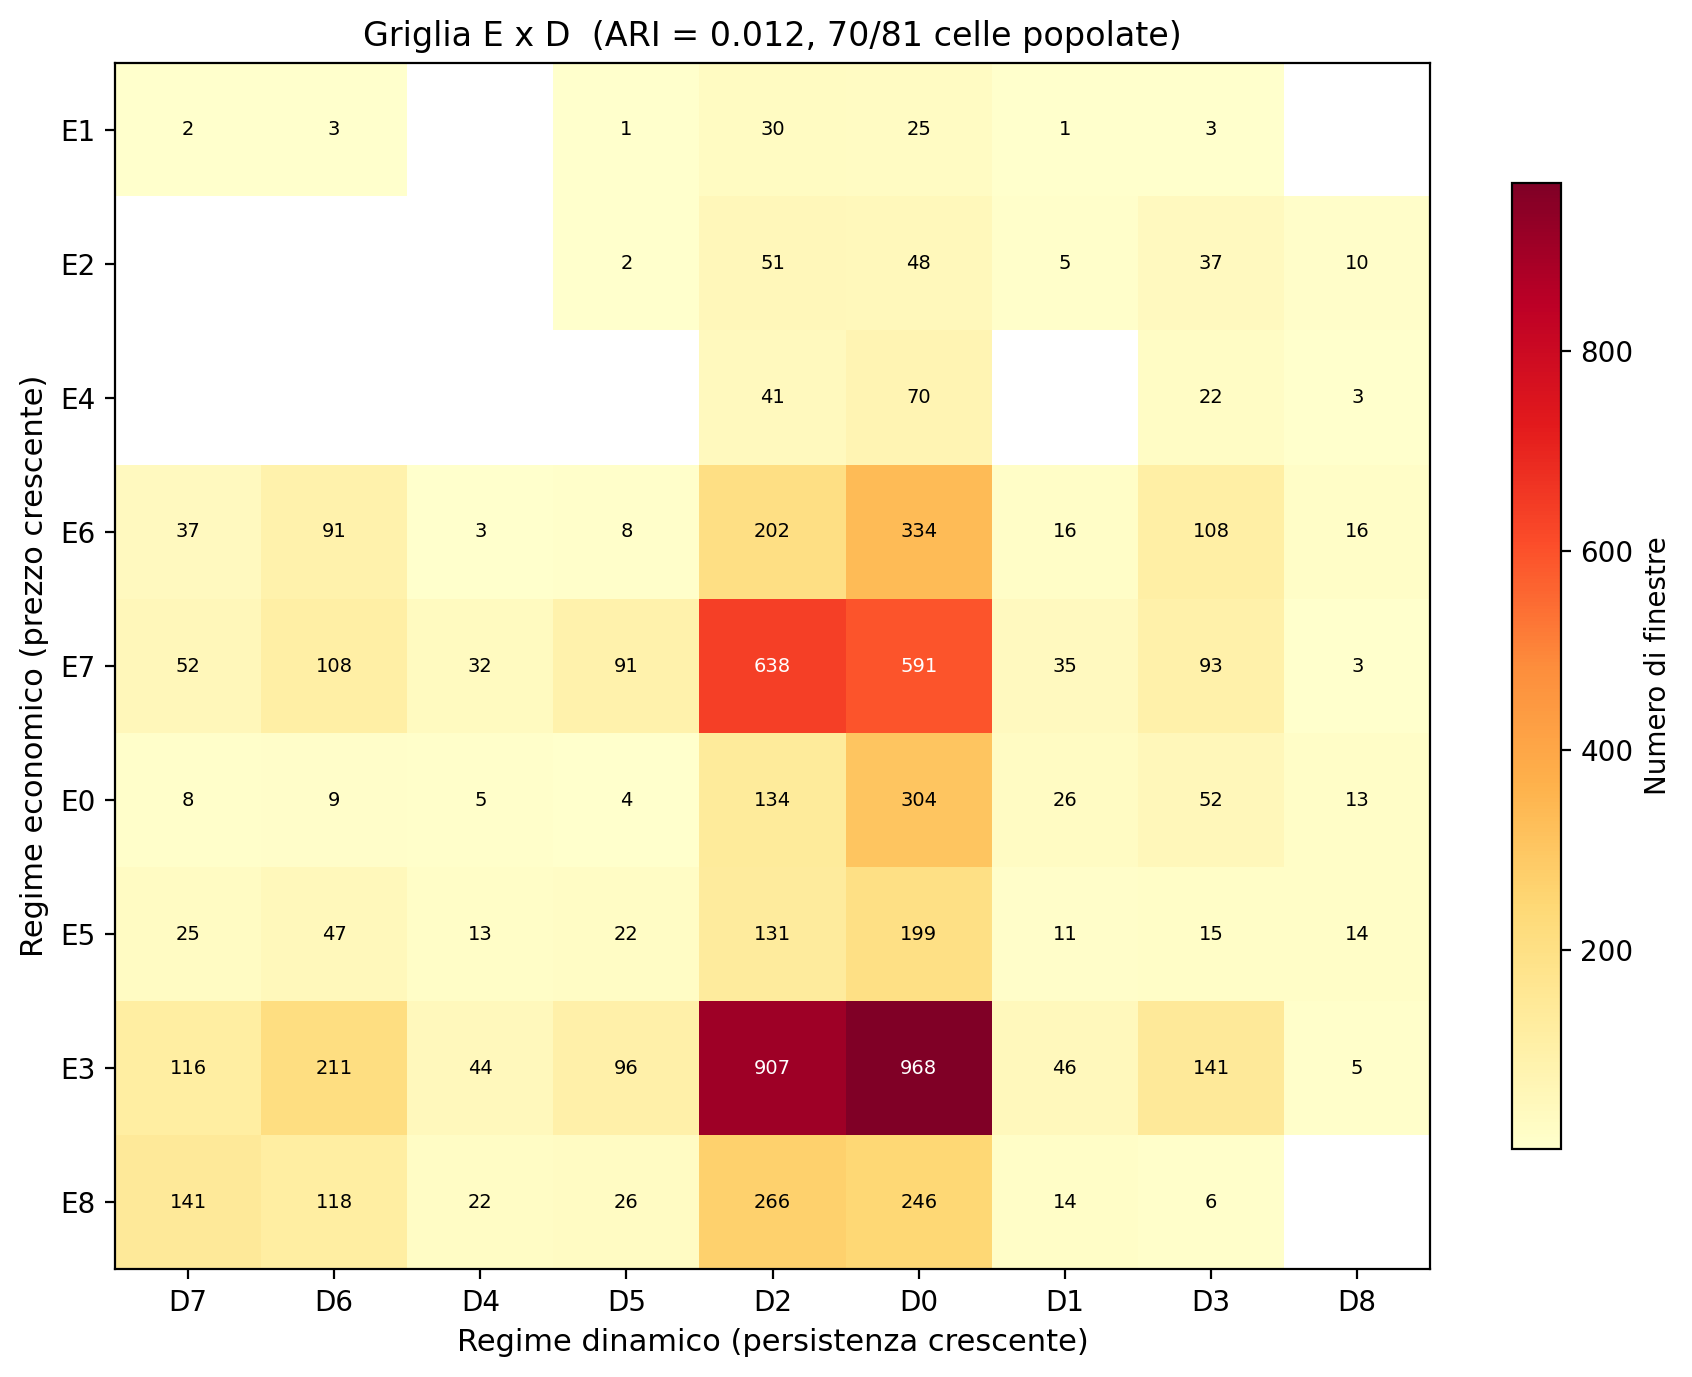
\includegraphics[width=0.65\textwidth]{ari_heatmap.png}
\caption{Heatmap della griglia $E \times D$. Ogni cella rappresenta una combinazione prezzo--persistenza; l'intensità del colore indica il numero di finestre. Se i due assi fossero ridondanti (ARI $\approx 1$), le finestre si concentrerebbero sulla diagonale. La distribuzione diffusa (70 celle su 81 popolate, ARI $= 0{,}012$) conferma che i due assi sono quasi ortogonali.}
\label{fig:ari_grid}
\end{figure}

Il valore dell'ARI è la prima evidenza a supporto della quasi-ortogonalità. La seconda è visiva.
La Figura~\ref{fig:axes_evidence} mostra ciascuna partizione contro ciascuna variabile di mercato in un layout $2\times 2$.
Il pannello~(a) mostra i regimi FE contro l'LMP: una scala monotona netta dove ogni regime occupa una banda di prezzo distinta --- FE separa il livello di prezzo.
Il pannello~(b) mostra i regimi MOMENT contro l'LMP: le distribuzioni si sovrappongono pesantemente, senza gradiente di prezzo --- MOMENT non separa il livello di prezzo.
Il pannello~(c) mostra i regimi MOMENT contro l'ACF al lag 6\,h: un gradiente monotono netto dalla rapida reversione allo sticky --- MOMENT separa la persistenza temporale.
Il pannello~(d) mostra i regimi FE contro l'ACF al lag 6\,h: distribuzioni piatte e sovrapposte --- FE non separa la persistenza.
Il pattern è diagonale: i pannelli~(a) e~(c) mostrano separazione netta, mentre i pannelli~(b) e~(d) no.
Ogni rappresentazione cattura una dimensione che l'altra in gran parte ignora.

\begin{figure}[H]
\centering
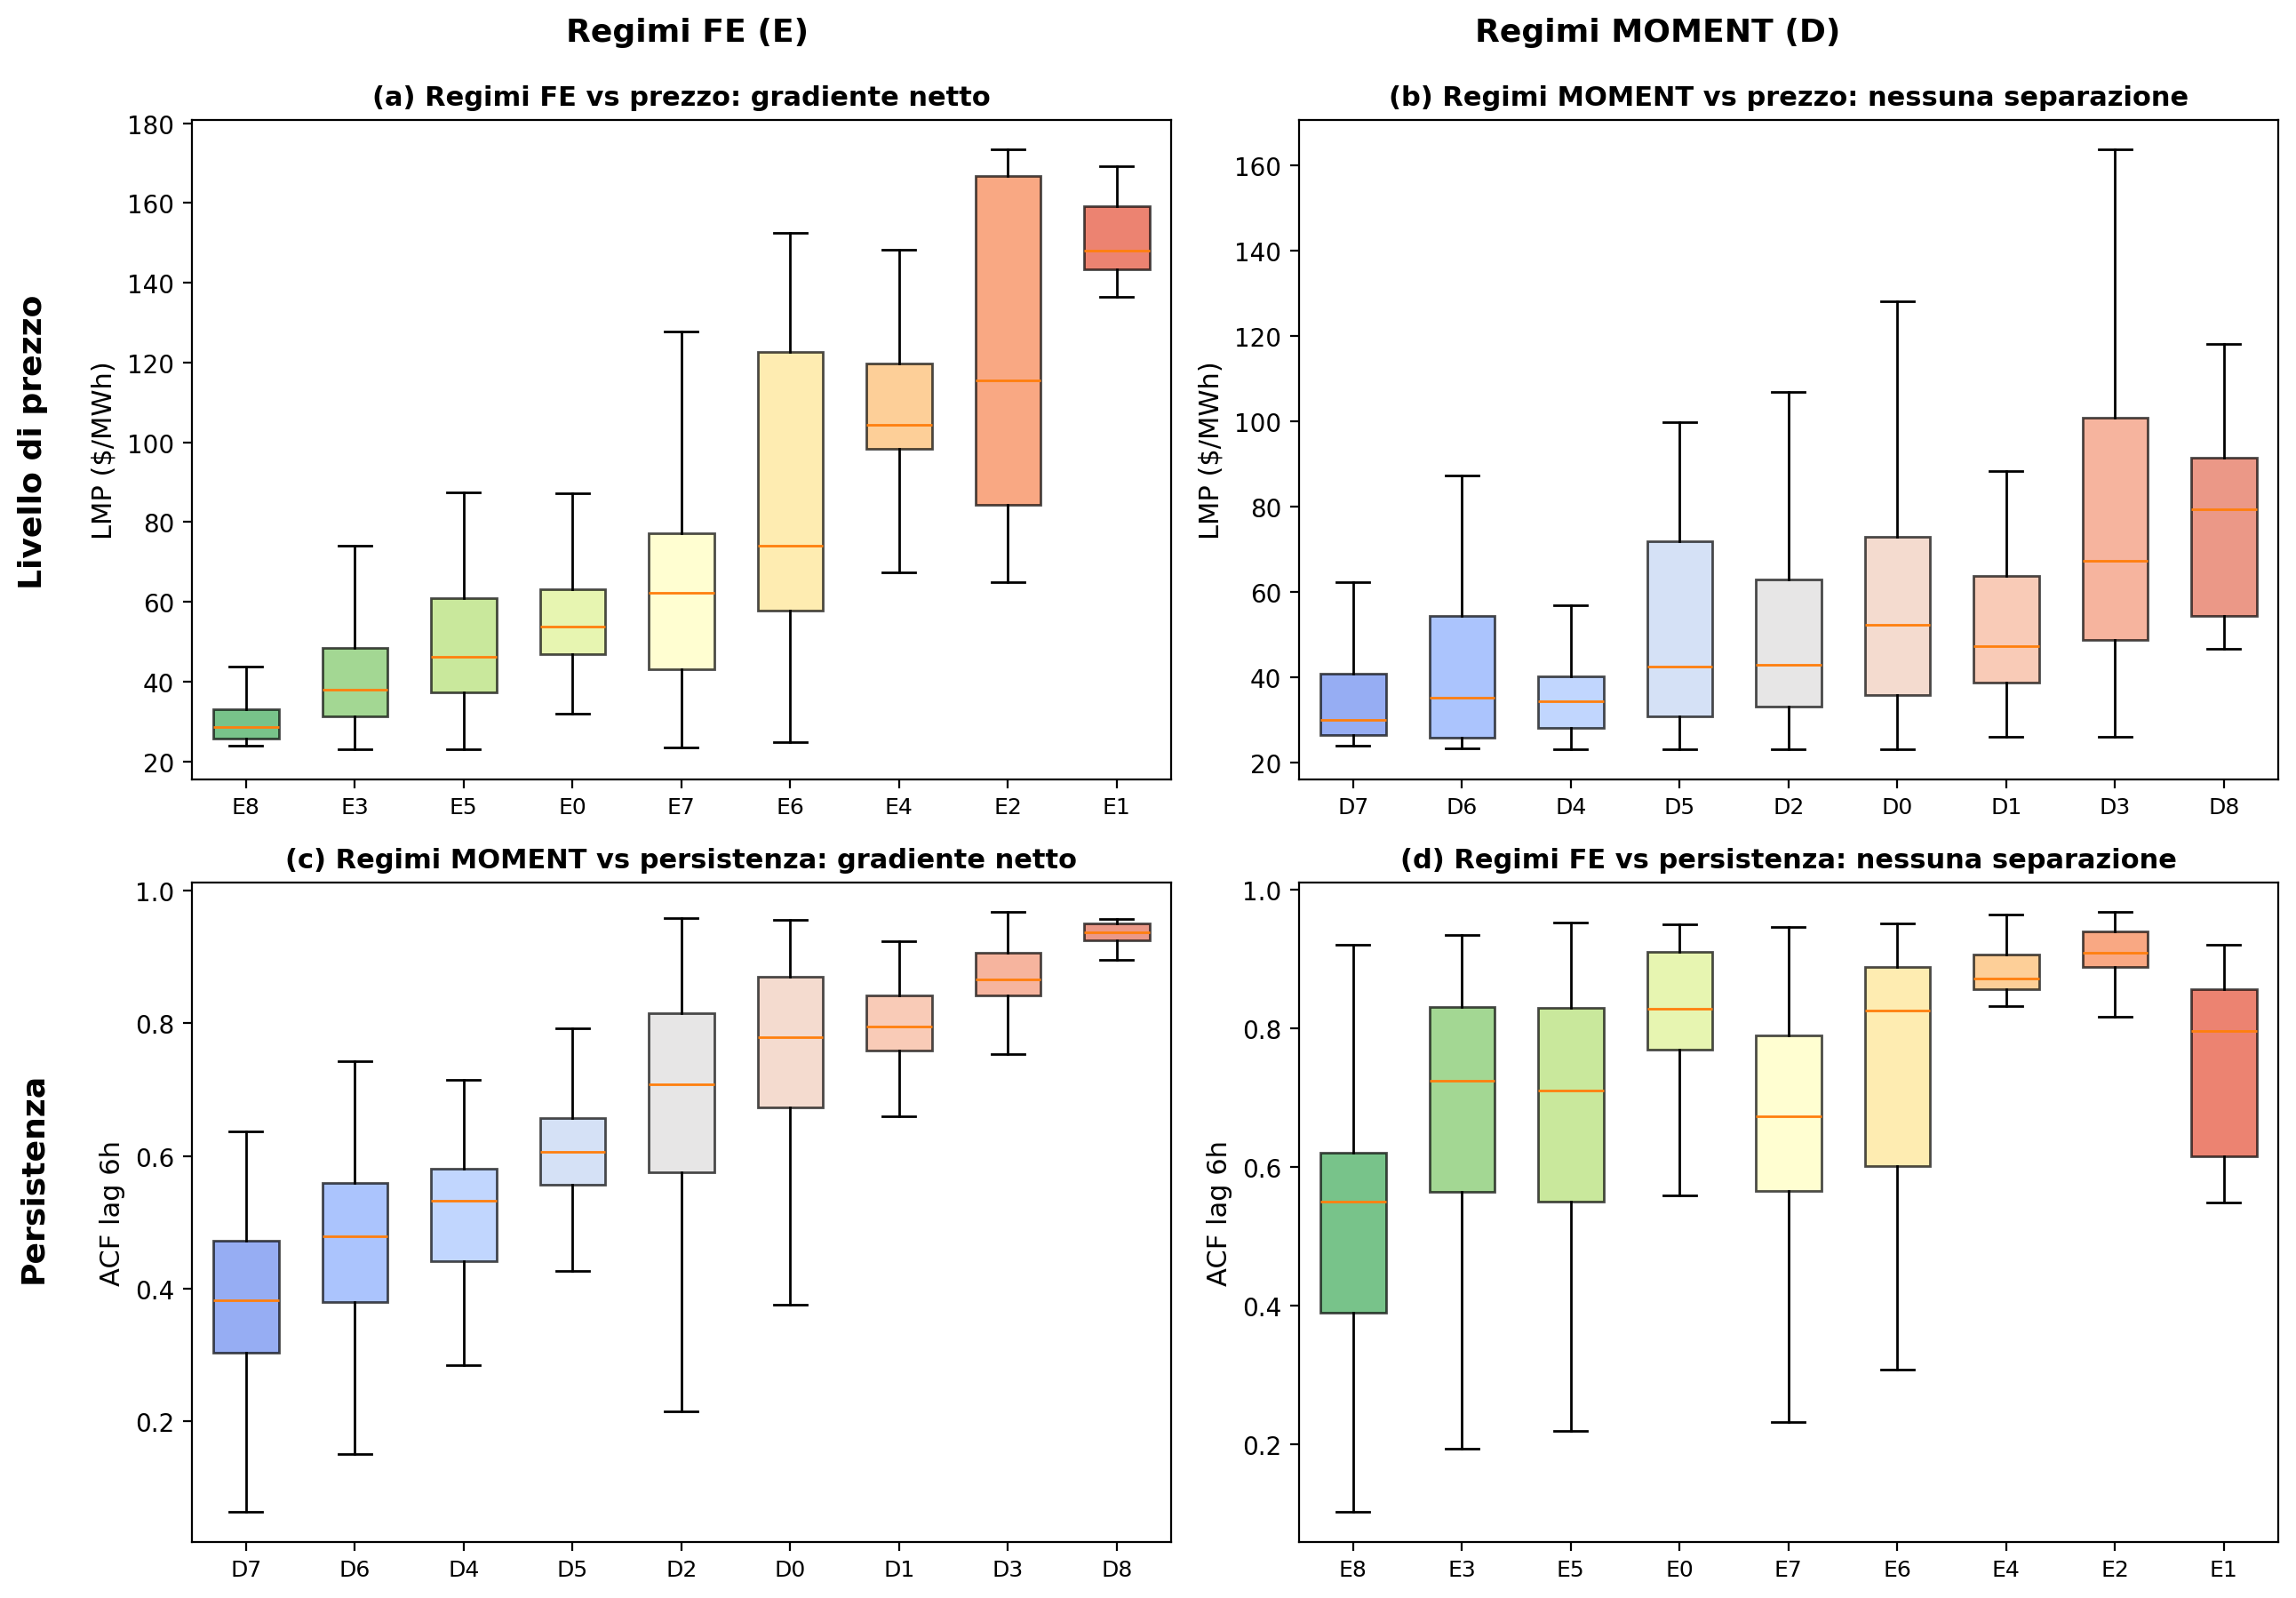
\includegraphics[width=\textwidth]{axes_evidence.png}
\caption{Ogni asse separa ciò che l'altro non può. (a)~I regimi FE producono un gradiente di prezzo monotono. (b)~I regimi MOMENT non separano il prezzo. (c)~I regimi MOMENT producono un gradiente di persistenza monotono. (d)~I regimi FE non separano la persistenza.}
\label{fig:axes_evidence}
\end{figure}

La quasi-ortogonalità dei due assi solleva una domanda immediata: questa struttura bidimensionale ha conseguenze pratiche, o è solo un'osservazione statistica?
Le sezioni seguenti dimostrano che l'omissione dell'asse dinamico --- la condizione operativa di tutti i modelli regime-switching che utilizzano un'unica etichetta di stato --- produce distorsioni sistematiche e quantificabili nell'allocazione del rischio.


% ── 4.4 Il modello a un asse è insufficiente ─────────────────────────────────
\subsection{Il modello a un asse è insufficiente}
\label{sec:model_insufficiency}

L'omissione dell'asse dinamico produce un \emph{underfitting locale della persistenza}: il modello è globalmente adeguato ma localmente distorto, con conseguenze invisibili alle metriche aggregate e visibili solo nell'analisi condizionata.

\subsubsection{Specificazione del modello}
\label{sec:model_spec}

\paragraph{Specificazione.}
Il residuo MSTL $r_t$ segue un processo mean-reverting verso zero:
\begin{equation}
r_t = (1 - \alpha)\, r_{t-1} + s_t, \qquad s_t \sim (0, \sigma_s^2),
\label{eq:mean_reverting}
\end{equation}
dove $\alpha \in (0, 1)$ è la velocità di mean-reversion e $s_t$ è la componente stocastica (innovazione).
Un valore di $\alpha$ vicino a zero indica che il processo è quasi un random walk (lo shock persiste indefinitamente); un valore vicino a uno indica una rapida mean-reversion.
La \emph{half-life} --- il tempo per dimezzare uno shock --- è $t_{1/2} = -\ln 2 / \ln(1-\alpha)$: con $\alpha = 0{,}15$, la half-life è di circa 4 ore.

\paragraph{Stima.}
Il parametro $\alpha$ è direttamente misurabile dall'autocorrelazione al lag~1 del residuo all'interno di ogni finestra di 512 ore:
\begin{equation}
\text{ACF}(1) \approx 1 - \alpha.
\label{eq:acf_alpha}
\end{equation}
Ogni finestra~$i$ ha il proprio $\hat{\alpha}_i = 1 - \widehat{\text{ACF}}_1(r_i)$, calcolato sui livelli $r_t$.
La volatilità del regime è misurata sugli incrementi: $\hat{\sigma}_i = \text{std}(\Delta r_i)$, calcolata sulla serie stazionaria $\Delta r_t$.
I parametri di una cella $(E, D)$ sono le medie delle finestre che vi appartengono:
\begin{equation}
\hat{\alpha}_{k,j} = \frac{1}{n_{k,j}} \sum_{i: e_i=k,\, d_i=j} \hat{\alpha}_i, \qquad
\hat{\sigma}_{k,j} = \frac{1}{n_{k,j}} \sum_{i: e_i=k,\, d_i=j} \hat{\sigma}_i.
\label{eq:cell_params}
\end{equation}

\paragraph{Perché queste variabili.}
La mean-reversion $\alpha$ è stimata sui livelli $r_t$ --- la variabile che MOMENT riceve e sulla quale i regimi $D$ sono definiti.
La volatilità $\sigma$ è stimata sugli incrementi $\Delta r_t$ --- la variabile stazionaria su cui FE opera.
Ogni parametro è misurato sulla variabile che lo cattura meglio, e l'unità di osservazione è la finestra ($N = 7\,217$), non la singola ora.

\paragraph{Due modelli a confronto.}
Confrontiamo due parametrizzazioni che differiscono nella granularità con cui $\alpha$ è stimato:
\begin{itemize}[nosep]
\item \textbf{Modello a un asse}: $\alpha(E)$, $\sigma(E)$ --- tutti i parametri sono mediati per regime economico $E$.
\item \textbf{Modello a due assi}: $\alpha(E,D)$, $\sigma(E,D)$ --- i parametri sono mediati per cella dello spazio congiunto.
\end{itemize}

\subsubsection{La mean-reversion varia dentro i regimi economici}
\label{sec:alpha_variation}

La Tabella~\ref{tab:alpha_range} riporta i risultati.
All'interno dello stesso regime economico, la velocità di mean-reversion $\alpha$ varia enormemente.
In $E_3$ (Baseload, \$41/MWh, il regime più grande con 2\,534 finestre), $\alpha$ va da 0,031 (half-life 22\,h --- lo shock persiste quasi un giorno) a 0,159 (half-life 4\,h --- lo shock si dimezza in mezza giornata).
Il modello a un asse assegna $\alpha(E_3) = 0{,}078$ (half-life 8,6\,h) a tutte le finestre: troppo lento per i transitori, troppo veloce per i persistenti.
La Figura~\ref{fig:alpha_heatmap} visualizza $\alpha$ nell'intero spazio $(E, D)$.

\begin{figure}[H]
\centering
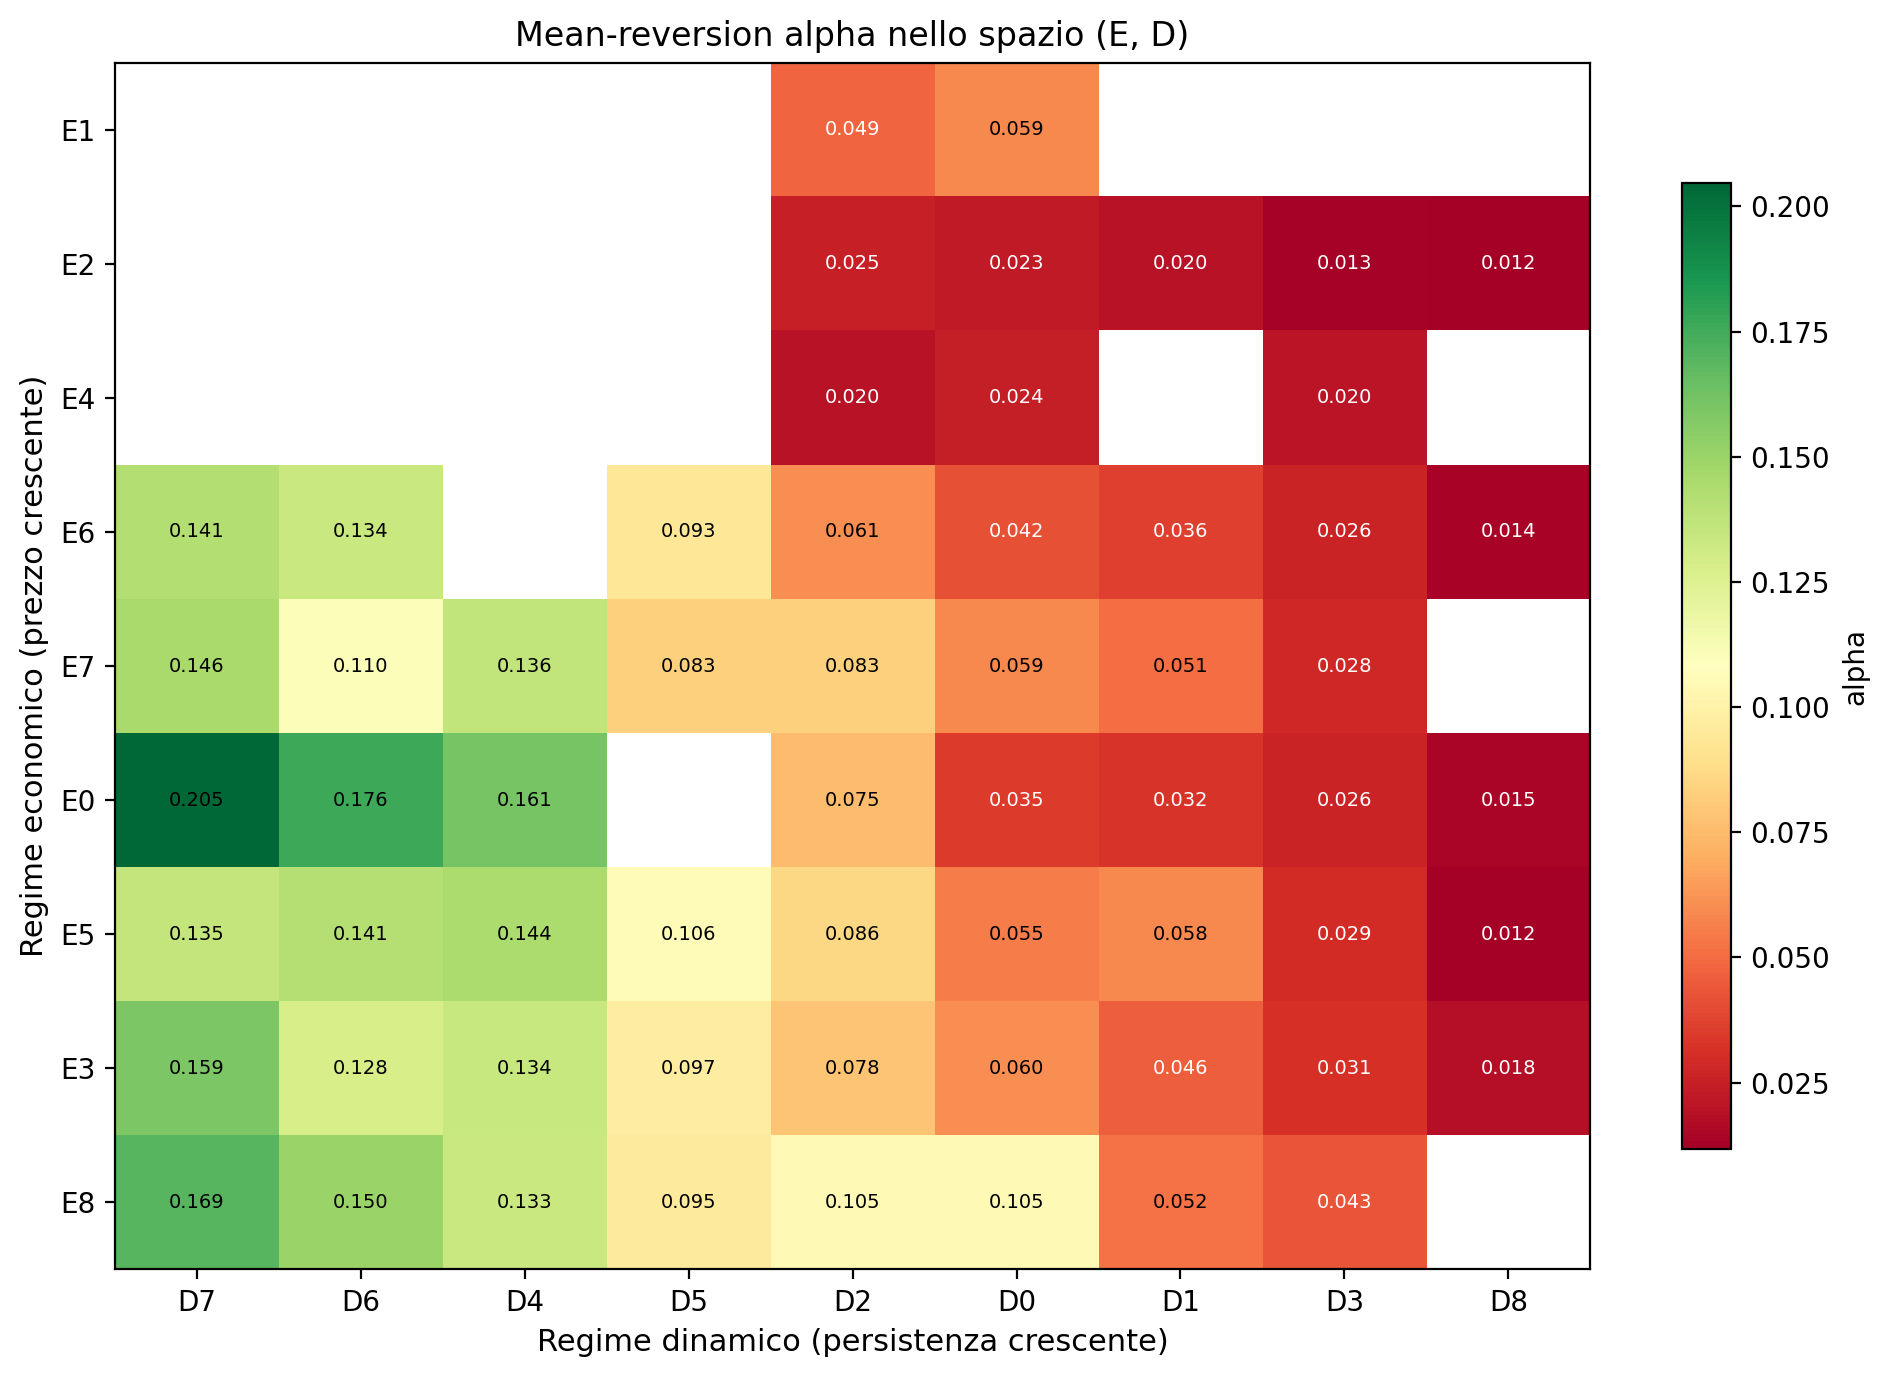
\includegraphics[width=0.85\textwidth]{alpha_heatmap.png}
\caption{Mean-reversion $\alpha$ nello spazio congiunto $(E, D)$. Verde = rapida reversione ($\alpha$ alto), rosso = persistente ($\alpha$ basso). Celle vuote = combinazioni non osservate.}
\label{fig:alpha_heatmap}
\end{figure}

\begin{table}[H]
\centering
\caption{Mean-reversion $\hat{\alpha}$ e volatilità $\hat{\sigma}(\Delta r)$ nei regimi $E$ principali.}
\label{tab:alpha_range}
\small
\begin{tabular}{lrrll}
\toprule
$E$ & $\alpha(E)$ & Half-life & Range $\alpha$ per $(E,D)$ & Range half-life \\
\midrule
$E_8$ (Off-peak, \$30) & 0,123 & 5,3\,h & 0,096--0,169 & 4\,h--7\,h \\
$E_3$ (Baseload, \$41) & 0,078 & 8,6\,h & 0,031--0,159 & 4\,h--22\,h \\
$E_0$ (Moderato, \$55) & 0,044 & 15,3\,h & 0,026--0,075 & 9\,h--26\,h \\
$E_7$ (Domanda, \$64) & 0,075 & 8,8\,h & 0,028--0,146 & 4\,h--24\,h \\
$E_6$ (Stress, \$84) & 0,060 & 11,2\,h & 0,026--0,141 & 5\,h--26\,h \\
$E_2$ (Spike inv., \$120) & 0,021 & 32,6\,h & 0,013--0,025 & 27\,h--53\,h \\
\bottomrule
\end{tabular}
\par\smallskip
\footnotesize\textit{Nota:} $\alpha(E)$ = valore unico del modello a un asse. Range = variazione tra celle $(E, D)$ dello stesso regime $E$.
Half-life $= -\ln 2 / \ln(1-\alpha)$. Ordinati per LMP crescente.
\end{table}

La Figura~\ref{fig:mc_trajectories} rende visiva la differenza.
All'interno dello stesso regime economico $E_3$ (Baseload, \$41/MWh), vengono campionate finestre empiriche da tre regimi dinamici con $\alpha$ diverso (riga superiore) e confrontate con traiettorie Monte Carlo simulate dal modello mean-reverting dell'Eq.~\eqref{eq:mean_reverting} con i parametri $\alpha$ e $\sigma$ della cella corrispondente (riga inferiore).
Le traiettorie a rapida reversione ($\alpha = 0{,}159$, half-life 4\,h) oscillano in una banda stretta attorno alla media; quelle persistenti ($\alpha = 0{,}031$, half-life 22\,h) presentano escursioni molto più ampie che impiegano quasi un giorno a rientrare.
La corrispondenza tra traiettorie empiriche e simulate conferma che il modello mean-reverting cattura la struttura dinamica essenziale, e che la variazione di $\alpha$ tra celle $(E, D)$ ha un significato fisico immediato.

\begin{figure}[H]
\centering

\includegraphics[width=\textwidth]{mc_trajectories.png}
\caption{Traiettorie empiriche (sopra, blu) e Monte Carlo simulate (sotto, rosso) per tre regimi dinamici all'interno di $E_3$ (Baseload, \$41/MWh). A sinistra: rapida reversione ($\alpha = 0{,}159$, half-life 4\,h). Al centro: moderata ($\alpha = 0{,}060$, half-life 11\,h). A destra: persistente ($\alpha = 0{,}031$, half-life 22\,h). Tutte le finestre provengono dallo stesso regime di prezzo ma mostrano dinamiche qualitativamente diverse.}
\label{fig:mc_trajectories}
\end{figure}

\paragraph{$D$ governa $\alpha$.}
Per quantificare quale asse governa la mean-reversion, calcoliamo l'$\eta^2$ su tutte le $N = 7\,217$ finestre.
L'asse $E$ da solo spiega il 16,1\% della varianza di $\alpha$; l'asse $D$ da solo ne spiega il 37,6\%; la partizione congiunta $(E, D)$ ne spiega il \textbf{46,6\%} --- un guadagno di 30 punti percentuali rispetto a $E$ solo.
La correlazione di Spearman tra il regime $D$ e l'$\alpha$ medio per cella è $\rho = 0{,}668$ ($p = 10^{-6}$): $D$ ordina i regimi per velocità di mean-reversion in modo altamente significativo.

La mean-reversion è primariamente una proprietà dell'asse dinamico, non di quello economico.
I modelli convenzionali che stimano la persistenza per regime di prezzo la attribuiscono all'asse sbagliato.

\paragraph{Confronto formale: BIC.}
Per verificare che l'eterogeneità di $\alpha$ non sia un artefatto della granularità, modelliamo $\alpha_i$ come gaussiano per cella e confrontiamo i due modelli via BIC \citep{schwarz1978}.
Il modello $E$ ha 18 parametri ($\mu_\alpha$ e $\sigma_\alpha$ per ciascun $E$); il modello $(E, D)$ ha 120 parametri.
Il risultato è $\Delta\text{BIC} = -3\,875$: il modello a due assi è schiacciante.
Per confronto, una differenza BIC di 10 è già considerata ``forte evidenza'' \citep{kass1995}.

\subsubsection{La volatilità nascosta}
\label{sec:sigma_variation}

Anche la volatilità degli incrementi $\sigma(\Delta r)$ varia dentro $E$, sebbene in misura minore ($\eta^2(E) = 0{,}29$, $\eta^2(E,D) = 0{,}36$, $\Delta\text{BIC} = -492$).
La Tabella~\ref{tab:sigma_range} riporta i range.

\begin{table}[H]
\centering
\caption{Range di $\sigma(\Delta r)$ dentro i regimi $E$ principali.}
\label{tab:sigma_range}
\small
\begin{tabular}{lrl}
\toprule
$E$ & $\sigma(E)$ & Range $\sigma$ per $(E,D)$ \\
\midrule
$E_8$ (Off-peak, \$30) & 0,069 & 0,058--0,072 \\
$E_3$ (Baseload, \$41) & 0,061 & 0,056--0,068 \\
$E_0$ (Moderato, \$55) & 0,077 & 0,071--0,080 \\
$E_6$ (Stress, \$84) & 0,053 & 0,044--0,057 \\
\bottomrule
\end{tabular}
\end{table}

\subsubsection{Efficienza allocativa del capitale}
\label{sec:risk_implications}

L'underfitting locale non è un'imperfezione statistica trascurabile: si traduce in una distorsione sistematica e \emph{asimmetrica} nell'allocazione del rischio.

Consideriamo il regime $E_3$ (Baseload, \$41/MWh, il più grande con 2\,534 finestre).
Il modello a un asse assegna $\alpha(E_3) = 0{,}078$ (half-life 8,6\,h) a tutte le finestre.
Ma dentro $E_3$, la half-life varia da 4\,h (regime $D$ a rapida reversione, $\alpha = 0{,}159$) a 22\,h (regime $D$ persistente, $\alpha = 0{,}031$) --- un fattore 5$\times$.
Le conseguenze operative sono opposte e simultanee:

\begin{itemize}[nosep]
\item \textbf{Nel sotto-regime a rapida reversione} ($\alpha \approx 0{,}16$, half-life $\approx 4$\,h).
Il modello a un asse applica $\alpha = 0{,}078$ (half-life 8,6\,h), sovrastimando la persistenza quasi del doppio.
Le coperture vengono calibrate su uno shock che nella realtà rientra in mezza giornata.
Il risultato è capitale immobilizzato inutilmente.

\item \textbf{Nel sotto-regime persistente} ($\alpha \approx 0{,}03$, half-life $\approx 22$\,h).
Il modello a un asse applica $\alpha = 0{,}078$ (half-life 8,6\,h), sottostimando la persistenza di un fattore 2,5$\times$.
Le posizioni di copertura risultano insufficienti proprio nei periodi in cui gli shock durano più di un giorno.
\end{itemize}

La distorsione è asimmetrica per costruzione: un unico $\alpha$ mediato produce \emph{simultaneamente} eccesso di copertura dove il mercato è calmo e carenza di copertura dove il mercato è sotto stress.
Questa inefficienza allocativa non è risolvibile affinando la stima di $\alpha(E)$: il problema non è nella precisione della stima, ma nel fatto che il parametro è vincolato a un asse che non lo governa.

\paragraph{L'asse D e la microstruttura del mercato.}
Dal punto di vista della microstruttura, un'interpretazione plausibile è che l'asse $D$ rifletta l'elasticità temporale dell'offerta e i vincoli operativi della rete, come congestioni, rampe di accensione dei generatori termici e inerzia del parco di generazione, fattori che sono per loro natura indipendenti dal livello nominale del prezzo.
Un mercato può trovarsi simultaneamente in un regime di prezzo elevato e in condizione di rapida mean-reversion (uno spike transitorio da picco di domanda che rientra in poche ore) oppure in un regime di prezzo moderato ma con persistenza elevata (un prolungato stress da offerta durante un'ondata di calore estiva).

Il modello convenzionale a singola etichetta di regime non è in grado di rappresentare queste combinazioni.
L'asse dinamico, scoperto dalla pipeline senza alcuna assunzione parametrica, fornisce la dimensione mancante e consente una caratterizzazione del rischio che va oltre il livello nominale di prezzo.


% ══════════════════════════════════════════════════════════════════════════════
% ── 4.5 Confronto con GARCH ──────────────────────────────────────────────────
\subsection{Confronto con GARCH}
\label{sec:garch}

Un benchmark naturale per la modellazione della varianza condizionata è la famiglia GARCH \citep{bollerslev1986}.
Stimiamo cinque varianti sulla serie completa degli incrementi $\Delta r_t$ ($N = 43\,811$), ciascuna con componente media AR(1): GARCH(1,1) con innovazioni normali, GARCH(1,1) con Student-$t$, GARCH(2,2) con Student-$t$, GJR-GARCH(1,1) con Student-$t$ (effetto leverage), ed EGARCH(1,1) con Student-$t$.
Per ciascun modello calcoliamo la volatilità condizionata $\sigma_t^\text{G}$, la aggreghiamo a livello di finestra (media su 512 ore) e misuriamo quanto essa si allinea con i regimi $E$ e $D$ tramite $\eta^2$.
La Tabella~\ref{tab:garch} riassume i risultati.

\begin{table}[H]
\centering
\caption{Confronto tra varianti GARCH. $\eta^2$ misura la quota di varianza della volatilità condizionata spiegata dai regimi.}
\label{tab:garch}
\small
\setlength{\tabcolsep}{4pt}
\begin{tabular}{lrrrrrr}
\toprule
Modello & $k$ & BIC & $\eta^2(E)$ & $\eta^2(D)$ & $\rho(\sigma^\text{G}\!,\alpha)$ & Kurt($z_t$) \\
\midrule
GARCH(1,1)-N        & 5 & 279\,286 & 0,285 & 0,020 & $-$0,02 & 4,77 \\
GARCH(1,1)-$t$      & 6 & 277\,462 & 0,286 & 0,020 & $-$0,02 & 4,82 \\
GARCH(2,2)-$t$      & 8 & 277\,452 & 0,287 & 0,020 & $-$0,02 & 4,81 \\
GJR-GARCH(1,1)-$t$  & 7 & 277\,463 & 0,288 & 0,021 & $-$0,02 & 4,80 \\
EGARCH(1,1)-$t$     & 6 & 277\,472 & 0,299 & 0,016 & $-$0,00 & 4,89 \\
\bottomrule
\end{tabular}
\par\smallskip
\footnotesize\textit{Nota}: $k$ = numero di parametri. $\rho(\sigma^\text{G}\!,\alpha)$ = correlazione tra la volatilità condizionata media per finestra e la velocità di mean-reversion $\alpha$ della finestra. Kurt($z_t$) = curtosi di Pearson dei residui standardizzati (gaussiana $= 3$).
\end{table}

Il pattern è uniforme attraverso tutte e cinque le specificazioni.
Ogni variante GARCH cattura parzialmente l'asse economico ($\eta^2(E) \approx 0{,}29$): le finestre ad alto prezzo tendono ad avere volatilità condizionata più elevata.
Tuttavia, \emph{nessuna} variante cattura l'asse dinamico: $\eta^2(D) \approx 0{,}02$ in tutti e cinque i casi, e la correlazione con la velocità di mean-reversion $\alpha$ è essenzialmente nulla.
Il test di Ljung-Box sui residui standardizzati al quadrato resta altamente significativo in tutti i modelli ($Q(24) > 800$, $p < 10^{-160}$), e la curtosi dei residui standardizzati ($\approx 4{,}8$) resta lontana dal valore gaussiano di 3.

Per confronto, il modello mean-reverting condizionato alla griglia $(E, D)$ (Sezione~\ref{sec:model_spec}) raggiunge $\eta^2(D) = 0{,}38$ sulla mean-reversion $\alpha$ e un $\Delta\text{BIC} = -3\,875$ rispetto al modello condizionato a $E$ solo.
La famiglia GARCH modella la \emph{volatilità} variabile nel tempo --- una proprietà che si allinea con l'asse economico --- ma è strutturalmente incapace di isolare la \emph{persistenza} temporale, che richiede la rappresentazione sequenziale del foundation model.
I due approcci catturano dimensioni ortogonali della serie: GARCH separa ``quanto grande è lo shock'', il modello a due assi separa anche ``quanto a lungo persiste''.



% ══════════════════════════════════════════════════════════════════════════════
\section{Discussione}
\label{sec:discussion}

La Tabella~\ref{tab:comparison} riassume i due assi prima di discuterne le implicazioni.

\begin{table}[H]
\centering
\caption{Caratterizzazione dei due assi.}
\label{tab:comparison}
\small
\begin{tabular}{lccccc}
\toprule
Asse & & $\eta^2$ & Trans.\% & Soggiorno & Tukey \\
\midrule
Economico (FE)   & $K_E = 9$ & 0,495$^\text{LMP}$  & 10,2\%  & 60\,h & 36/36 \\
Dinamico (MOMENT) & $K_D = 9$ & 0,420$^\text{ACF}$  & ---  & ---  & --- \\
\bottomrule
\end{tabular}

\medskip
\small
\textit{Nota}: $\eta^2$ è calcolato sui 9 regimi finali sulla variabile target primaria (LMP per l'economico, ACF al lag 6\,h per il dinamico); i valori coincidono con la Tabella~\ref{tab:cross_projection} perché anche la diagnostica di separazione è calcolata sulla partizione post-merge.
Trans.\% = tasso di transizione alla risoluzione di 6 ore; Soggiorno = tempo di soggiorno medio; Tukey = coppie significative / coppie totali ($\alpha = 0{,}05$) sulla variabile target primaria.
Le metriche temporali dell'asse dinamico non sono riportate perché i regimi $D$, definiti sulla persistenza e non sul livello, non presentano la stessa stabilità temporale dell'asse $E$.
\end{table}

I due assi hanno conseguenze pratiche dirette.
L'asse economico risponde a \emph{quanto} costa l'elettricità; l'asse dinamico risponde a \emph{come} si comporterà il prezzo nelle ore e nei giorni successivi.
Tutte e quattro le combinazioni di prezzo alto/basso e mean-reversion rapida/lenta sono popolate (Figura~\ref{fig:quadrants}), ciascuna con un significato operativo distinto.
Gli stati ad alto prezzo e rapida reversione (18\% delle finestre) sono spike transitori che si risolvono rapidamente; una copertura aggressiva pagherebbe troppo.
Gli stati ad alto prezzo e shock-persistenti (32\%) sono eventi di stress prolungati, tipicamente ondate di freddo invernale, dove la copertura è giustificata e le riserve di emergenza possono esaurirsi.
Gli stati a basso prezzo e rapida reversione (32\%) sono mercati calmi con clima mite dove le operazioni normali sono sufficienti.
Gli stati a basso prezzo e sticky (18\%) sono periodi prolungati di prezzi moderati o bassi dove il rischio di curtailment delle rinnovabili è elevato e gli operatori di stoccaggio dovrebbero caricare.
Un'etichetta convenzionale a singolo asse ``spike'' raggruppa eventi ad alto prezzo transitori e persistenti, anche se i loro profili di rischio sono qualitativamente diversi.

\begin{figure}[H]
\centering

\includegraphics[width=0.65\textwidth]{two_axis_grid.png}
\caption{Spazio dei regimi a due assi. Ogni punto è una finestra, posizionata per LMP medio (asse orizzontale) e ACF al lag 6\,h (asse verticale). I quattro quadranti (prezzo alto/basso $\times$ persistenza alta/bassa) sono tutti popolati, confermando che le due dimensioni variano indipendentemente.}
\label{fig:quadrants}
\end{figure}

% --- Perché MOMENT cattura le dinamiche ---

Una domanda importante è \emph{perché} MOMENT separi la persistenza temporale mentre le feature costruite manualmente no.
Il punto di partenza è che il residuo MSTL conserva una forte dipendenza seriale (ACF lag~1 $= 0{,}977$, Tabella~\ref{tab:acf}): il preprocessing rimuove i cicli stagionali ma preserva la persistenza a breve termine che distingue le diverse dinamiche di mercato.
Questa persistenza è la materia prima che entrambe le rappresentazioni ricevono, ma la elaborano in modo molto diverso.
FE opera sugli incrementi $\Delta r_t$ (stazionari): le sue feature distribuzionali catturano la forma degli shock, non la persistenza temporale --- e per costruzione non include feature ACF, che sarebbero prossime a zero sugli incrementi (Sezione~\ref{sec:repr_fe}).
MOMENT, al contrario, riceve i livelli $r_t$ (persistenti, ACF lag~1 $= 0{,}977$) e codifica la struttura temporale come suo segnale \emph{primario}: il suo obiettivo di pre-addestramento basato sulla ricostruzione mascherata (\emph{masked time-series modeling}) forza l'encoder del transformer ad analizzare i pattern nel loro contesto temporale, rendendolo architetturalmente idoneo a intercettare e codificare proprio le variazioni della memoria stocastica che gli incrementi eliminano.
Come dimostrato nella Sezione~\ref{sec:model_insufficiency}, questa capacità si traduce in un asse di persistenza che governa il parametro di mean-reversion $\alpha$ ($\Delta\text{BIC} = -3\,875$) e che nessuna combinazione di feature distribuzionali è in grado di isolare.
L'embedding MOMENT a 1\,024 dimensioni si riduce a 5 coordinate di diffusione (gap spettrale, Sezione~\ref{sec:diffmaps}), confermando che il foundation model organizza le sue rappresentazioni lungo un numero ridotto di modi temporali dominanti.

% --- Relazione con la letteratura esistente ---

La struttura a due assi si connette alla letteratura sul regime-switching in modo nuovo.
Gli approcci classici basati su HMM assumono un singolo stato latente che guida simultaneamente sia il livello di prezzo sia la dinamica della volatilità.
La nostra scoperta suggerisce che questa assunzione potrebbe essere troppo restrittiva: livello e persistenza sembrano essere governati da processi latenti indipendenti.
Un mercato può trovarsi in un regime economico ad alto prezzo e in un regime dinamico a rapida reversione simultaneamente --- una combinazione che un HMM a catena singola non può rappresentare senza un'espansione esponenziale dello spazio degli stati.

% --- Validazione e limitazioni ---

Il framework di validazione è deliberatamente multidimensionale: Tukey HSD assicura la distinzione statistica all'interno di ciascun asse, e la coerenza temporale dell'asse economico (tempi di soggiorno di $\sim$60\,h, transizioni prevalentemente tra adiacenti) conferma che i regimi di prezzo riflettono dinamiche fisiche di mercato piuttosto che artefatti statistici.
Nessuna singola metrica scalare può confrontare adeguatamente una partizione che separa livelli di prezzo con una che separa dinamiche temporali; la diagnostica di separazione (Tabella~\ref{tab:cross_projection}) e l'ARI quasi nullo stabiliscono insieme che i due assi catturano aspetti genuinamente diversi della struttura di mercato.

% --- Perché solo il prezzo ---

La pipeline opera deliberatamente solo su dati di prezzo.
Nei mercati all'ingrosso competitivi, l'LMP aggrega già le informazioni dal lato dell'offerta e della domanda tramite il dispacciamento merit-order: uno spike del gas, una siccità eolica o un guasto a un generatore si manifestano tutti nell'LMP prima di apparire in qualsiasi variabile esogena.
Variabili esogene (temperatura, prezzi spot del gas, errori di previsione delle rinnovabili) potrebbero rivelare ulteriori dimensioni ortogonali, e il framework cross-ARI fornisce lo strumento per testarlo: qualsiasi nuova rappresentazione che produca una partizione con ARI quasi nullo rispetto a entrambi gli assi noti costituirebbe una genuina terza dimensione della struttura di mercato.

% --- Limitazioni ---

Diverse limitazioni devono essere riconosciute.
Le finestre scorrevoli sovrapposte ($S/W = 6/512$) inflazionano la dimensione campionaria nominale; il numero effettivo di finestre indipendenti di 21 giorni è circa 85.
La partizione economica a 9 regimi rappresenta un taglio a grana fine di un gradiente di prezzo continuo; il numero di regimi distinguibili dipende dalla potenza statistica, ma il gradiente monotono e la significatività di tutte le coppie sono preservati.
L'analisi copre un singolo mercato (ISONE) e nodo di prezzo; la generalizzazione ad altri ISO richiede ulteriori studi.
Il foundation model è applicato zero-shot; un fine-tuning specifico per il dominio potrebbe rafforzare l'asse dinamico.
La finestra di 512 ore impone una scala temporale minima, e la pipeline è retrospettiva; la previsione dei regimi in tempo reale resta un lavoro futuro.

% ══════════════════════════════════════════════════════════════════════════════

\section{Conclusioni}
\label{sec:conclusion}

Questo lavoro introduce una pipeline non parametrica per il rilevamento non supervisionato dei regimi nei mercati elettrici spot, in cui il numero di regimi e la dimensionalità effettiva delle rappresentazioni emergono dai dati attraverso l'analisi della persistenza topologica.
Applicando questa pipeline a cinque anni di prezzi orari di ISO New England con due rappresentazioni alternative, arriviamo a una scoperta strutturale: il mercato elettrico è organizzato lungo almeno due assi quasi ortogonali di struttura dei regimi.

Il primo asse è economico: 15 feature, di cui 11 distribuzionali e una di volatilità infragiornaliera sugli incrementi $\Delta r_t$, più 3 statistiche sull'LMP grezzo, producono $K_E = 9$ regimi che vanno dall'off-peak allo spike estremo invernale.
Questi regimi persistono per giorni e transitano gradualmente attraverso livelli di prezzo adiacenti.

Il secondo asse è dinamico: MOMENT, operando sui livelli $r_t$, produce $K_D = 9$ regimi separati per persistenza temporale --- quanto rapidamente avviene la mean-reversion dopo uno shock.
$K_E$ e $K_D$ emergono dalla stessa pipeline senza alcun intervento esterno.
I due assi sono quasi ortogonali.

Nessuna singola rappresentazione è sufficiente: i regimi economici servono la copertura, i regimi dinamici servono la previsione, e i due devono essere impiegati in parallelo.

La pipeline (Diffusion Maps, ToMATo e merge Tukey HSD) fornisce una metodologia rigorosa e riproducibile che non richiede alcuna assunzione a priori sul numero di stati di mercato e può essere direttamente trasferita ad altri mercati e serie di prezzi di materie prime.
Il framework cross-ARI qui introdotto fornisce anche uno strumento per il lavoro futuro: qualsiasi nuova rappresentazione (feature nel dominio delle frequenze, embedding multivariati, variabili esogene) che produca una partizione con ARI quasi nullo rispetto a entrambi gli assi noti costituirebbe una genuina aggiunta alla dimensionalità della struttura di mercato.

% ══════════════════════════════════════════════════════════════════════════════
\bibliographystyle{plainnat}
\bibliography{references}

\end{document}
